% Created 2020-08-04 Tue 16:17
% Intended LaTeX compiler: pdflatex

% \author{Nicholas Knoblauch}
% \date{\today}
\chapter{FGEM}


% \maketitle
% \setcounter{tocdepth}{2}
% \tableofcontents


\section{Introduction}\label{sec:org28fe636}

%The goal in mapping the genetic basis of a complex trait is to identify the genetic variants that meaningfully perturb the activity of the genes that act in the pathways that are relevant to the trait of interest.  
Geneticists often aggregate genetic evidence of variants within a gene to test if the gene is related to a trait of interest. These gene-level tests are among the most powerful and commonly used tools in the geneticist's toolkit for relating genotype to phenotype.
Gene-based tests have been used in many contexts, including Genomewide association studies, Transcriptome- wide association studies \cite{predixcan}, rare variant analysis from exome sequencing studies \cite{skat}, rare variant analysis in family data \cite{TADA}, and cancer driver gene discovery using somatic mutations \cite{drivermaps}. In fact, almost all methods for genetic analysis using very rare mutations, including de novo germline and somatic mutations, are gene-based, as it is almost impossible to identify individual causative mutations. %One shortcoming of gene-based tests and indeed of all association-based tests is that if there is insufficient power (e.g due to small sample size) the test may lead to a
%false negative.  Conversely, if the gene-based test has inadequate false discovery rate (FDR) control, use of the test may lead to false positives. 

There is often advantages in performing gene-level test in a Bayesian framework. Variants inside a gene often have very different functionalities, e.g. nonsense mutations can be highly deleterious while missense mutations can have very different effects depending on where they are located. Similarly, for tests that combine different types of variants in a gene, such as common and rare variants, it is important to consider different effects of these variants, with rare variants generally having more deleterious effects. While frequentist methods in theory can use different weights for different groups of variants in the test, it is difficult in practice to know what weights should use. Bayesian statistical framework allows researchers to effectively combine evidence of different sets of variants, by using different effect size distributions. Importantly, these distributions can be estimated from data using Empirical Bayes framework or fully Bayesian Inference using MCMC. The power of Bayesian approach to gene-based analysis has been demonstrated in very different contexts. Transmission and De novo Association test (TADA) and its extensions \cite{TADA} are widely used to analyze variants from sequencing studies in parent-child trios, by effectively combining de noov and inherited variants to improve the power. DriverMAPS is a recently developed method for identifying signatures of positive selection in cancer driven genes, with the strength of selection varying across positions in a gene depending on functional information of the positions\cite{drivermaps}. The results of Bayesian gene-based analysis are often summarized as Bayes factors, which compares the model where the gene has an effect on phenotype (causal model) vs. non-causal model.  

A common followup after identifying a set of putative causal genes is pathway analysis, which tests if certain biological pathways are enriched in these genes \cite{rss-e}\cite{Carbonetto_2013}\cite{Lamparter_2016}. This approach is supported by the evidence that the functions of genes underlying complex traits, including cancer, often converge on certain biological processes. In the simplest form, pathway analyses apply a cutoff on trait-associated genes, and then use Fisher's enrichment test for pathways overrepresented in the genes passing the cutoff. More sophisticated analysis would compare the distribution of trait associations in genes in a pathway and those outside the pathway. Pathway analysis is an important tool for geneticists to learn possible biological mechanisms by which the putative causal genes may acting to influence the trait of interest. This information can provide guidance in deciding on which genes are the most likely to replicate, and most worthy of follow-up \cite{Hou_2013}.

Gene-level test and pathway analysis are generally treated as separate problems. An interesting possibility is to combine the two, in particular, using the pathway enrichment results to set informative prior in Bayesian gene-level test. Conceptually, if a gene belongs to a disease-related pathway, then a priori, the gene is more likely to be a disease gene. Incorporating this prior would thus improve our power of identifying disease risk genes. This possibility has been demonstrated in earlier work on GWAS variant-level analysis. In fgwas, for example, a variant is annotated by functional information such as conservation and enhancer marks, and the method learns the enrichment of these annotations in putative causal variants and uses these results to set prior probabilities of association of variants. Similar idea has also been used for gene-based analysis in GWAS, where gene annotations are based on pathways \cite{Carbonetto_2013}. All these methods, however, are specifically designed for GWAS, and cannot be used for other gene-based analysis, e.g. those based on rare variants or somatic mutations. Additionally, for the gene-based GWAS analysis, they can only incorporate prior from a single annotation, while in reality, multiple pathways/annotations may be informative.  

%Gene-level prior information can combined with a gene-level summary of the evidence under causal and non-causal scenarios (the Bayes factor) to arrive at a gene-level posterior proability that a gene is causal.  While there is an increasing wealth of gene-level information through databases such as the Gene Ontology\cite{GO}, translating this information into a gene-level prior is not straightforward.
We propose a method for combining gene-level evidence, as summarized by Bayes factors, with one or more gene-level annotations to jointly estimate the global enrichment of the annotations, and to re-estimate a gene-level posterior conditional on the estimated enrichment estimates. We call this method \texttt{FGEM}. The method is easy to use, requiring only a set of Bayes factors from gene-level analysis and functional annotations of the genes. This generality makes the method, and our software, useful for a wide variety of settings.    
FGEM is related to frequestist methods that control false discovery rate or family-wise error rate while weighing different hypothesis using external information. However, these methods cannot be applied to the Bayesian setting, which, as we argued, has advantages in gene-based tests. 
%Previous approaches have attempted to incorporate gene-level covariate information to adjust the false discovery rate at the
%SNP-level\cite{Zablocki_2014}, but do not directly reprioritize genes, or can only incorporate a single annotation at a time\cite{rss-e}.  
We demonstrate the power of the \texttt{FGEM} model by applying it to the problem of
identifying mutational cancer driver genes. We use the gene-based Bayes factors generated by the \texttt{driverMAPS} method, as applied to 18 cancer types from The Cancer Genome Atlas
(TCGA) data\cite{TCGA}\cite{drivermaps}, and use the Gene Ontology Biological Processes as gene-level annotations.

% By aggregating evidence over multiple variants, inonsistencies that can arise from population differences can be more readily resolved\cite{Neale_2004}
% While \texttt{driverMAPS} incorporates base-pair level functional annotation, functional annotation at the gene level is ignored.  There is an extremely rich body of gene-level functional annotation.  Among the most extensive corpora of gene-level annotation is the Gene Ontology\cite{GO}.  The Gene Ontology uses a controlled vocabulary for describing the properties of genes (specifically gene products).  The three domains of the Gene Ontology are cellular component, which correspond to the various parts of the cell(e.g the ribosome), molecular function, which correspond to the biochemical activities of a gene product (e.g protein kinase activity), and biological process, also known as ``biological programs'', are higher-level, coordinated molecular activities (e.g DNA repair).

\section{Method}\label{sec:org4822ac5}

%The task of assigning a prior probability directly from gene-level annotation is not straightforward.  The total number of causal genes is in general not known (though in the case of mutational driver genes, the total number is believed to be in the hundreds\cite{Bailey_2018}), nor is there a comprehensive set of properties that a causal gene must have (or not have).  To circumvent this problem, 
FGEM uses an empirical Bayes approach to construct the \emph{a priori} probability that a gene is causal, based on the annotations of genes.The method uses genetic data (summarized as gene-level Bayes factors or likelihood ratios) and a set of gene-level annotations to inform which annotations are relevant and to what extent.
% When identifying mutational driver genes with FGEM, we applied the model to the data from each cancer type separately.  What follows is a description of the model as applied to genetic data from a single cancer type.
\subsection{FGEM Model}\label{sec:org4e93496}

For each gene  \(g \in \{1 \dots G\}\), let the indicator variable \(z_g=1\) denote that gene \(g\) is causaully related to the trait or disease of interest.  The evidence for and against the hypothesis that \(z_g=1\) can be
summarized using a bayes factor:

$$B_g=\frac{P(x_g|z_g=1)}{P(x_g|z_g=0)}$$

where \(x_g\) is the subset of a length $G$ vector of genetic data corresponding to the $g$th gene.

Let \(F\) be the number of features for which functional annotations are available for each of our \(G\) genes.  Let \(\textbf{a}_g\) denote the length \(F\) vector of annotations for gene \(g\), and \(\textbf{A}\) denote the matrix with \(F\) rows and \(G\) 
columns consisting of \(\textbf{a}_1 ...  \textbf{a}_G\)
We define the prior probability of $z_g$ as a logistic function of the annotations of $g$:

$$\pi(\boldsymbol{\beta}, \textbf{a}_g) =  P(z_g=1|\textbf{a}_g,\boldsymbol{\beta}) =  \frac{1}{1+e^{-(\beta_{0}+\sum_{f=1}^F{A_{f,g}\beta_f})}} $$

The likelihood of \(\boldsymbol{\beta}\) is computed by treating the data from each gene as coming from a two component mixture model (where \(z_g=1\) and where \(z_g=0\)) and marginalizing over the two components:

$$ P(\textbf{x}|\boldsymbol{\beta},\textbf{A})=\prod_{g=1}^{G}P(x_g|\boldsymbol{\beta})=\prod_{g=1}^{G}[\pi(\boldsymbol{\beta},\textbf{a}_g) P(x_g|z_g=1)+(1-\pi(\boldsymbol{\beta},\textbf{a}_g))P(x_g|z_g=0)]$$

By factorizing out the term \(\prod_{g=1}^{G} P(x_g|z_g=0)\) (which does not depend on $\boldsymbol{\beta}$), the likelihood for \(\boldsymbol{\beta}\) (up to a constant of proportionality) can be expressed in terms of \(\textbf{B}\):

\begin{equation}
P(\textbf{x}|\boldsymbol{\beta},\textbf{A}) \propto \prod_{g=1}^{G}[\pi(\boldsymbol{\beta},\textbf{a}_g)B_g+(1-\pi(\boldsymbol{\beta},\textbf{a}_g))]
\label{eq:FGEM_lik}
\end{equation}


Given a particular value of \(\boldsymbol{\beta}\), and a bayes factor \(B_g\),  the posterior probability that \(z_g=1\) is given by:

$$P(z_g=1 | B_g, \boldsymbol{\beta},\textbf{a}_g) = \frac{\pi(\boldsymbol{\beta},\textbf{a}_g) B_g}{\pi(\boldsymbol{\beta} , \textbf{a}_g) B_g + 1 - \pi(\boldsymbol{\beta},\textbf{a}_g)}$$


The goal of the FGEM method is to simultaneously estimate the enrichment $\boldsymbol{\beta}$ for a relevant set of features and the gene-level posterior probability \(P(Z_g=1|\textbf{a}_g,\boldsymbol{\beta},x_g)\) that each gene is causally related to the trait of interest. FGEM estimate $\boldsymbol{\beta}$ by maximizing the log-likelihood, given by Equation~\ref{eq:FGEM_lik}. Given an estimate of $\boldsymbol{\beta}$ it is straightforward to compute
\(P(Z_g=1|\textbf{a}_g,\boldsymbol{\beta},x_g)\).

When the number of annotations is large, it is impossible, from both a computationally and interpretability standpoint, to include all features in the model.
Furthermore, as the number of features in the model increases, the probability that some subset of features will be collinear with one-another increases,
which can complicate model-fitting, as \(\boldsymbol{\beta}\) becomes unidentifiable. This is especially important when a binary, hierarchical feature set
like the Gene Ontology.  To avoid these issues, FGEM maximizes the penalized log-likelihood, in a multi-stage feature-selection and model fitting procedure. In the first step, all
single-feature-plus-intercept models are fit, and a \$p\$-value is obtained for each model by comparing the single-feature-plus-intercept model to the intercept-only model via the
likelihood ratio test.  From this set of single-feature models, all of the nonsignificant (i.e features with Benjamini-Hochberg adjusted
\$p\$-values greater than 0.05) features were removed from the analysis.

%\subsubsection{Joint Model}\label{sec:orga62a234}

In the second step, significant features passing the filter were combined in a joint model and fit by maximizing the log-likelihood, penalized with an elastic-net penalty.  The Limited Memory Broyden-Fletcher-Goldfarb-Shanno algorithm (LM-BFGS)\cite{LMBFGS} is among the most popular algorithms
for unconstrained optimization over scalar, differentiable functions, and while suitable for the un-penalized single-feature plus intercept models, cannot be used in the penalized setting without modification.  One limitation of LM-BFGS, is that the function that is being optimized must be differentiable.  Unfortunately, sparsity-inducing $l_{\text{1}}$-regularized models of the form:

$$f(\boldsymbol{\theta})=p(\boldsymbol{\theta} | \textbf{x}) + C \Vert \boldsymbol{\theta} \Vert_1$$ are not differentiable when any of the elements of the parameter vector $(\boldsymbol{\theta})$ are 0.  The Orthant-wise limited-memory quasi-Newton method is a variant of LM-BFGS which is designed precisely for fitting $L_1$-regularized, sparsity inducing models.  FGEM utilizes the Orthant-wise LM-BFGS algorithm to maximize the marginalized likelihood in the presence of a non-zero $l_{\text{1}}$ penalty.
%\subsubsection{Regularization by (relaxed) elastic-net}\label{sec:orge3a8031}

The multi-feature fitting procedure consists of two steps.  In the first step, the objective function corresponding to the negative of the elastic-net penalized log-likelihood:
$$ -\mathcal{L}(\textbf{x}|\boldsymbol{\beta},\textbf{A}) + \lambda\left( \frac{1-\alpha}{2} \sum_{j=2}^F\beta_j^2 + \alpha \sum_{j=2}^F|\beta_j| \right) $$
is minimized, where \(\mathcal{L}(\textbf{x}|\boldsymbol{\beta},\textbf{A}) = \sum_{g=1}^{G}[\log\left(\pi(\boldsymbol{\beta},\textbf{a}_g)B_g+(1-\pi(\boldsymbol{\beta},\textbf{a}_g))\right)]\).
 

The overall level of sparsity in the model is controlled by the parameter \(\lambda\), while the proportion of \(l_1\) vs \(l_2\) penalty is determined by \(\alpha\).  For this first step FGEM uses a default value of $\alpha=0.95$, corresponding to a higher $l_{\text{1}}$ penalty relative to the $l_{\text{2}}$ penalty, which has the effect of encouraging sparsity in the model. The objective function is maximized at 100 values of \(\lambda\), starting at zero, and ending at \(\lambda_{\text{max}}\), equally spaced on a log scale.  \(\lambda_{\text{max}}\) is defined as the smallest value of \(\lambda\) for which the objective function is minimized, and all coefficients but the intercept are 0 (the intercept term is not subject to the elastic net penalty). The optimal value of \(\lambda\) is chosen using 10-fold cross-validation.  

In the second step, features with \(\beta_f=0\) are removed from the analysis, and cross-validation over 100 values of \(\lambda\) occurs again, this time with \(\alpha = 0\), meaning there is no \(l1\) penalty.  The motivation for this two-stage
procedure comes from the "relaxed" lasso\cite{hastie17_exten_compar_best_subset_selec}, wherein the lasso is used for feature selection, and the model is refit without a lasso penalty.  

\subsubsection{Removal of highly enriched features}\label{sec:org02cff25}

    A subset of features were removed after the single-feature feature-selection stage as they exhibited very high enrichment estimates, and when incorporated in multi-feature models, these features tended to have high multi-feature enrichment estimates. One consequence of FGEM's latent variable approach is that it is possible to encounter a scenario analogous to the ``separation'' problem in logistic regression.  In logistic regression, if one (or several) predictors predict an output perfectly, the likelihood for that feature is not maximized at a finite parameter value, which can result in extremely high enrichment estimates.  Because there is a high level of redundancy in the Gene Ontology feature-set, little information is lost by excluding these problematic features. To choose a threshold of enrichment parameter $\beta$, we compute the prior probability of a gene, if it has that feature. If this prior $> 0.3$, we think this enrichment is too high, and we will remove that feature from consideration for inclusion in the joint model (these features were included when calculating the FDR-adjusted p-values for the single-feature tests).  

\subsubsection{Comparison with Fisher's Exact test}\label{sec:orge6f1632}

In the case of a single binary feature, one can apply a Bayes Factor cutoff to obtain a contingency table and assess the enrichment of the feature using Fisher's Exact test.
We compared FGEM with Fisher's exact test, using an FDR cutoff of 0.1, and compared the $p$-values to those obtained from the single-feature, likelihood ratio test FGEM $p$-values.

\subsection{Genetic Data from The Cancer Genome Atlas and \texttt{driverMAPS}}\label{sec:org31ff9f1}

The Cancer Genome Atlas (TCGA) is a resource consisting of data on over 20 cancer types, gathered from thousands of individuals\cite{TCGA}.  For several cancer types TCGA data include high coverage, whole-exome sequencing data for both the patient's solid tumor and matched adjacent normal tissue. By aggregating the somatic mutation data across multiple individuals with a particular cancer type, one can identify a set of genes that undergo somatic mutation at a frequency higher than expected by chance.  For each of 18 TCGA cancer types, we used 20,848 gene-level Bayes factors obtained from running the statistical method \texttt{driverMAPS}, a recently developed Bayesian method for identifying driver genes, as input to the FGEM model.  After obtaining the total set of gene-level Bayes factors, we eliminated ``blacklisted'' genes known to have mapping problems\cite{drivermapsblacklist}, as well as Olfactory Receptors, which are also known to have mappability problems\cite{Derrien_2012}.

\subsection{Gene-Level Annotations using Gene Ontology}\label{sec:orgd117550}

The "Biological Process" gene sets from the Gene Ontology were obtained using the Bioconductor package \texttt{GO.db}\cite{godb}. Of the 10,930 possible biological process gene ontology terms, the 2,198 terms that 
include 10 or more genes were deemed elegible for incorporation in this analysis, so as to reduce the multiple testing burden, and to ensure that we were well powered to accurately estimate the enrichment of each term included in the analysis.  Each gene ontology term was encoded as a binary, gene-level feature using an indicator variable to indicate a gene's association with the corresponding term. 

\subsection{Validation of predicted cancer genes using external resources}\label{sec:orgd8b4e10}

IntOGen is a database of cancer driver genes\cite{gonzalez-perez13_intog_mutat_ident_cancer_driver}.  It is populated by an ensemble method that incorporates seven different methods for identifying cancer driver genes.  
It weights each of the 7 methods according to their ability to predict membership in the The Catalogue of Somatic Mutations in Cancer (COSMIC) Cancer Gene Census (CGC)\cite{COSMIC}.
To validate the FGEM models, we compared the posterior under the functional model to the functional posterior under the uniform model.

\subsection{FGEM Software Package}\label{sec:org56b3320}

Our method is distributed as a freely available R package\cite{Rlang} \texttt{FGEM}, which is available at the 
GitHub repository \texttt{https://github.com/CreRecombinase/FGEM}.  In addition to the implementing an optimized version of the FGEM
likelihood itself, the package also has afforadances for both
single-feature (single-annotation) and multi-feature (multiple annotation) model fitting.  FGEM relies on both the \texttt{RcppEigen}\cite{RcppEigen} and  \texttt{StanHeaders} R
packages for efficient computation of the likelihood and its gradients, which are passed to the optimizer routine.  

\section{Results}\label{sec:org6fb4837}

\begin{figure}[h]
  \centering
  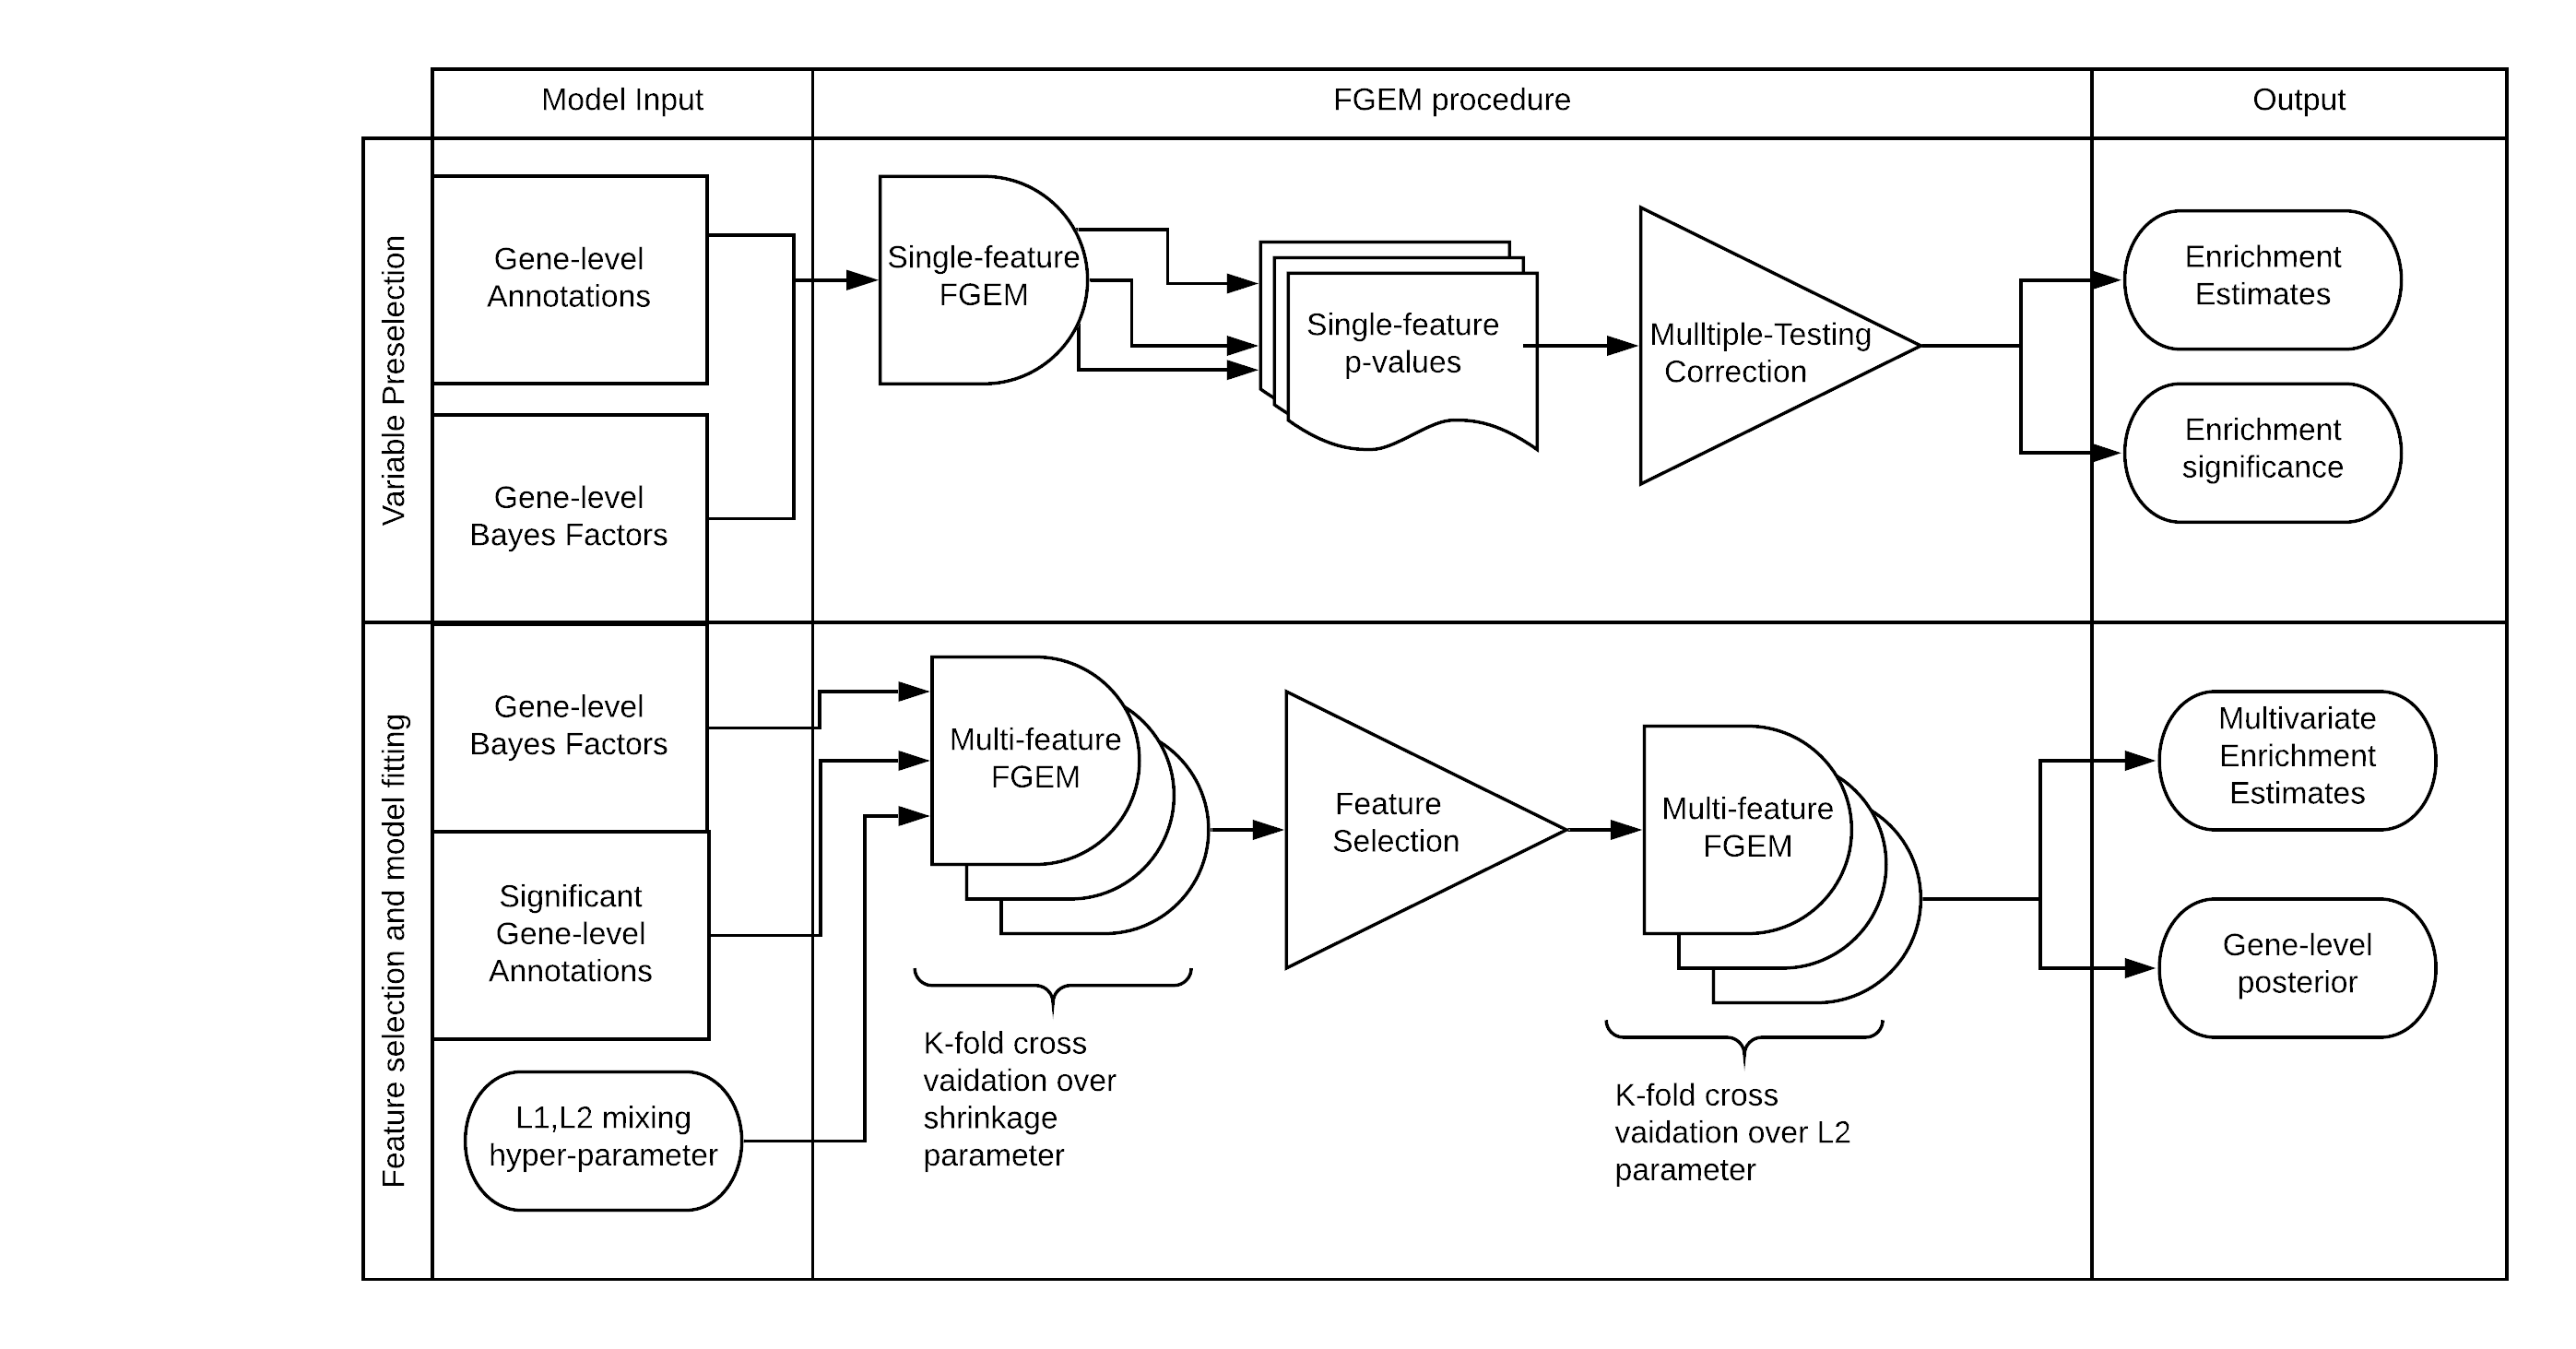
\includegraphics[width=.9\linewidth]{img/FGEM_procedure.png}
  \label{fig:overview}
  \caption{Overview of the FGEM procedure for gene-set enrichment and gene mapping.  In the preliminary feature pre-selection phase, all single-feature models are fit, and $p$-values are obtained for each model.
    Features with FDR-adjusted $p$-value less than a significance cutoff (0.1) are incorporated in the multi-feature model. The multi-feature model is fit with an elastic-net penalty, with a user-specified proportion of $l_1$
    to $l_2$ penalty ($\alpha$), and $k$-fold cross-validation to determine the optimal penalty parameter ($\lambda_{\text{opt}}$).  The subset of features with non-zero enrichment estimates under the model with the selected $\lambda_{\text{opt}}$ undergo a final round of $l_2$ only $k$-fold cross-validation (i.e relaxed elastic-net).  The final $l_2$ penalized multi-feature enrichment estimates are then used to generate gene-level posteriors. }
\end{figure}


\subsection{A probabilistic framework for gene-set enrichment and gene prioritization applied to cancer gene discovery}\label{sec:org2d4ff20}

Our approach is outlined in ~\ref{fig:overview}. In brief, we combine gene-level Bayes factors summarizing the hypothesis that a gene is causally related to a trait of interest with gene-level annotations about that gene to identify the properties causal genes are likely to have, and simultaneously re-estimate the gene-level posterior probability that the gene is causal.  Let $Z_g$ be and indicator variable with $Z_g = 1$ indicating that gene $g$ is causally related to the trait of interest, and $Z_g = 0$ indicating that it is not.  While $Z_g$ is unobserved, the evidence for and against $Z_g=1$, as calculated by a gene-based test on some body of genetic evidence, is summarized by the Bayes factor for that gene $B_g$.  FGEM incorporates gene-level annotation, represented as an $F$ (the total number of gene-level features) by $G$ (the total number of genes) matrix $\textbf{A}$. FGEM relates $Z_g$ to $\textbf{A}$ through a length $F$  enrichment parameter $\boldsymbol{\beta}$.  For a particular gene $g$, $P(z_g=1|\textbf{a}_g,\boldsymbol{\beta}) =  \frac{1}{1+e^{-(\beta_{0}+\sum_{f=1}^F{A_{f,g}\beta_f})}} $.  This relationship between feature and and response is analagous to a logistic regression on a latent variable ($\textbf{Z}$).  The procedure for model fitting is described in the Methods section\ref{sec:org4822ac5}.

Under the single-feature FGEM model, in which each feature is considered one at at time, if the value of $\beta$ for a binary gene-level annotation is greater than $0$, this indicates that genes with this annotation have a higher probability of being causal to the trait of interest than background genes.  %Similarly, an estimate of $0$ indicates that the genes with the feature have the same probability of being causally related to the trait of interest as genes without the annotation.  
It is also possible for the estimate of $\beta$ to be less than $0$, indicating that the genes with the annotation have a lower probability of causal association than random genes.  The statistical significance of a single feature is assessed using the likelihood ratio test, testing if $\beta = 0$, from which $p$-values were calculated.

For a particular value of $\boldsymbol{\beta}$ (and $\textbf{A}$), we can compute a new value for $(Z_g = 1 | \textbf{A},\boldsymbol{\beta})$.
% Under the FGEM model, we model $P(Z_g = 1 | \textbf{A},\boldsymbol{\beta})$.
We refer to the value of $\beta_a$ as the enrichment of feature $a$.  For each of the 18 TCGA cancer types, we fit a single-feature model for each of the 2,657 Biological Process related GO terms.  We refer to the value of $\beta$ for each feature when fit one at a time as single-feature enrichment.  Significant features for each cancer type were then jointly fit for each cancer type.  The estimated value of $\beta$ for each feature under this model is referred to as the multi-feature enrichment, and the procedure for obtaining multi-feature enrichment estimates is described in the Methods section\ref{sec:orge3a8031}.

\begin{figure}
\centering
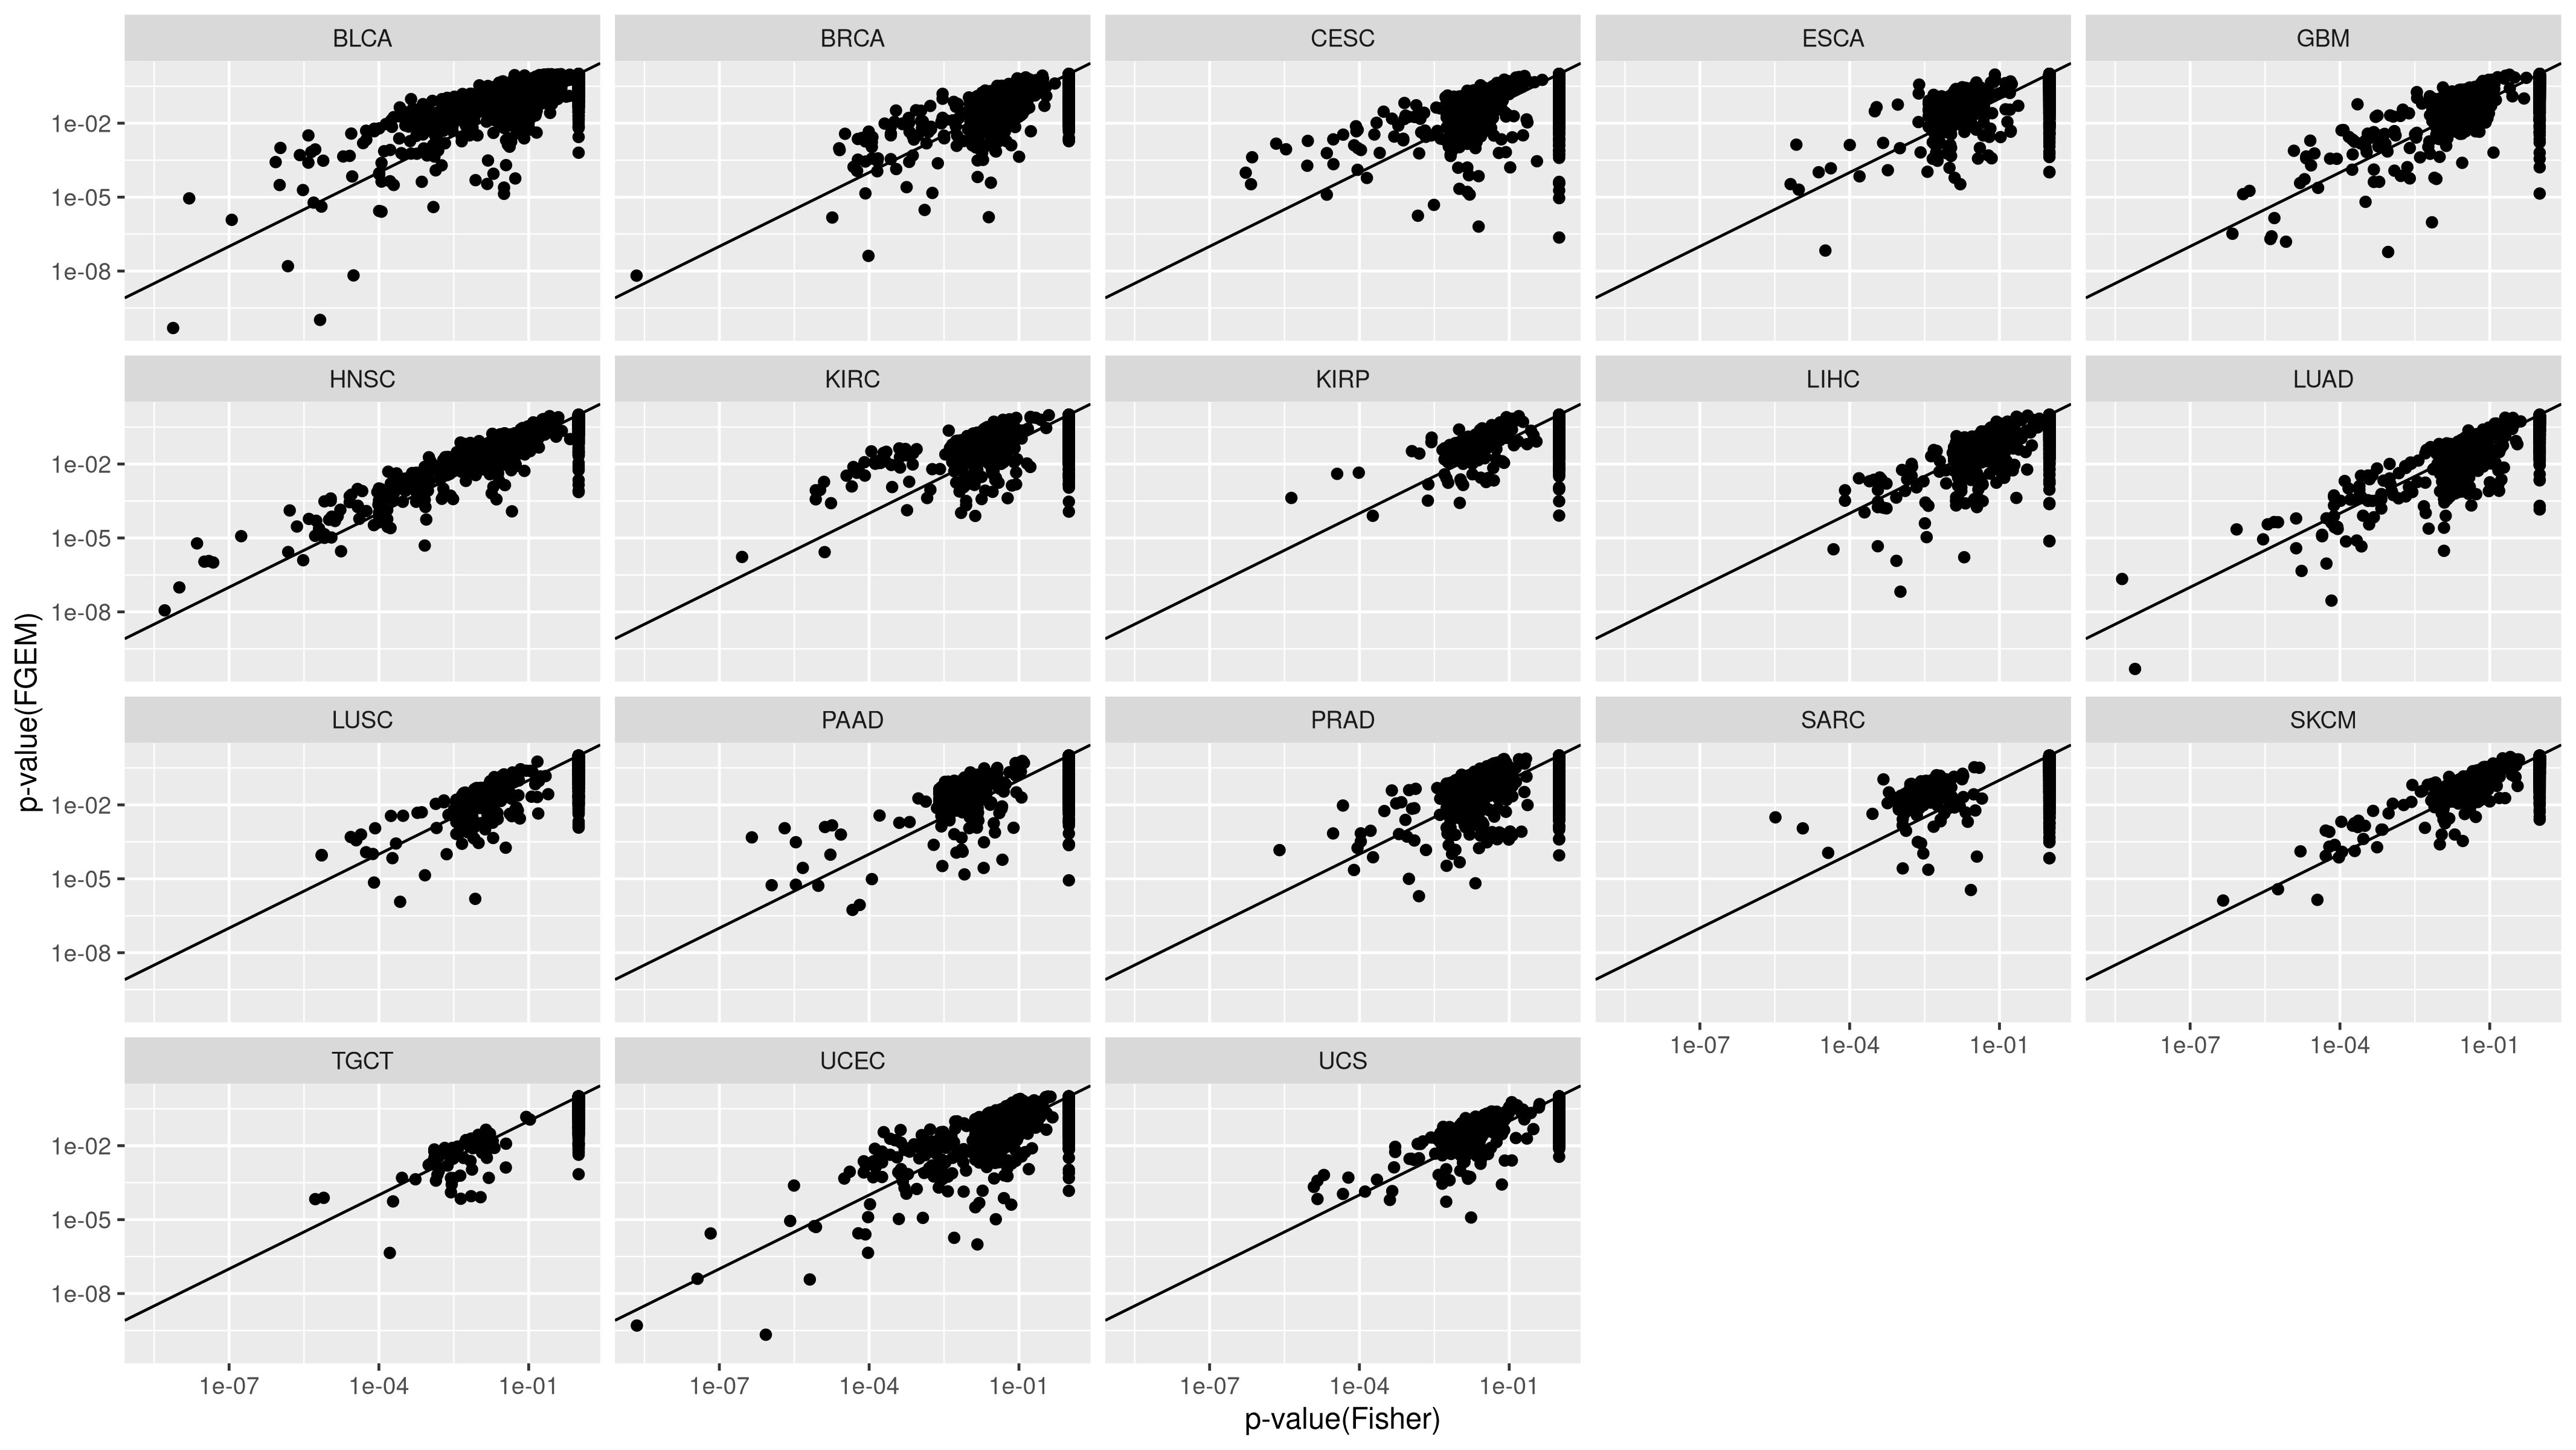
\includegraphics[width=.9\linewidth]{img/fisher_vs_fgem.png}\label{fig:fisher_vs_fgem}
\caption{Comparison of single-feature FGEM and Fisher's exact test $p$-values for 18 TCGA cancer types.}
\end{figure}

\subsection{Recurrent enriched annotations reflect the hallmarks of cancer}\label{sec:orgd52f2ca}

After removing Gene Ontology Biological Process features with a small number of annotated genes, there were 2,657 features.  Evaluating the enrichment of each of these features in a single-feature fashion with the 18 TCGA cancer types resulted 47,826 single-feature enrichment estimates. We first evaluated the number of significantly enriched features, stratified by cancer type.  With a false discovery rate (FDR) of $0.01$, all cancer types but KIRP and UCS had at least one (i.e 16 out of 18) significant association, with HNSC having the most, at 38.\ref{tab:single-featureFDR}.  With a relaxed FDR of $0.15$, all 18 cancer types had at least one significantly associated feature\ref{tab:single-featureFDR}. In all cancer types analyzed, all features with enrichments significantly different from 0 (at all tested FDR) were positively enriched.  

We next compare our single feature analysis with a simple Fisher's exact test, which uses a cutoff to define candidate genes, and tests enrichment of a pathway in all genes passing the cutoff. Overall, we see clear correlation of the results of these two tests (Figure~\ref{fig:fisher_vs_fgem}, however, one notable difference is that a number of features with small p-values by FGEM single feature model have p-values equal to 1 under FET - see the data points close to the vertical y-axis in Figure~\ref{fig:fisher_vs_fgem}. This counter-intuitive results can be explained by the fact that with a hard cutoff, many gene sets will have no genes passing the cutoff, so will be missed by FET. Since FGEM treats gene status $z_g$ as latent variable to be marginalized out, avoiding the hard cutoff, it is possible to identify these gene sets. 

\begin{table}
  \centering
  \begin{tabular}{l|r|r|r|r}
    \hline
    cancer & FDR$=0.01$ & FDR$=0.05$ & FDR=$0.1$ & FDR=$0.2$ \\
    \hline
    HNSC & 38 & 95 & 122 & 209\\
    
    LUAD & 31 & 77 & 111 & 190\\
    
    BLCA & 26 & 51 & 67 & 110\\
    
    UCEC & 22 & 52 & 92 & 141\\
    
    GBM & 20 & 42 & 55 & 99\\
    
    CESC & 14 & 36 & 67 & 115\\
    
    PAAD & 11 & 22 & 32 & 54\\
    
    BRCA & 8 & 26 & 37 & 82\\
    
    LIHC & 8 & 33 & 55 & 95\\
    
    LUSC & 4 & 11 & 24 & 53\\
    
    PRAD & 3 & 15 & 50 & 131\\
    
    SKCM & 3 & 8 & 14 & 26\\
    
    KIRC & 2 & 2 & 14 & 53\\
    
    ESCA & 1 & 13 & 31 & 54\\
    
    SARC & 1 & 8 & 14 & 29\\
    
    TGCT & 1 & 8 & 15 & 27\\
    
    KIRP & 0 & 0 & 0 & 6\\
    
    UCS & 0 & 4 & 20 & 23\\
    
  \end{tabular}\label{tab:single-featureFDR}
  \caption{Number of significantly enriched features in single-feature enrichment test at four False Discovery Rates.}
\end{table}

We identified a set of recurrent features: features that were significantly enriched in more than one cancer type.  We characterized 161 Gene Ontology features as significantly enriched in more than one cancer type, and 50 features were significantly enriched in 5 or more cancer types.  The top features ranked by the number cancer types in which the feature was enriched \ref{tab:sig_single-feature} recapitulates almost all of the 10 ``Hallmarks of cancer''
\cite{Hanahan_2011}.  The feature with the highest mean (and median) enrichment is GO:2000774, positive regulation of cellular senescence, with a median enrichment estimate of 5.458, and a mean enrichment estiamte of 7.91.  %In a third of cancer types analyzed (6 of the 18), the univarite, FDR-adjusted $p$-value for GO:2000774 was less than 0.1.  The relevance of this feature to cancer is obvious and bordering on tautalogical: 
This feature is important for tumorigenesis: mutations in genes that prevent cells from entering oncogene induced cellular senscence (especially those related to the ARF/TP53 pathway) are essential for progression of almost all cancers\cite{chandeck10_oncog_induc_cellul_senes}.  %It is difficult to overstate the importance of positive regulation of cellular senescence as a key guard against cancer.  Indeed, TP53 had the highest average log Bayes Factor of all genes going in to the analysis, and had the highest average posterior probability of being a cancer gene as a result of the analysis, reinforcing the finding that regulators of cellular senescence, and those in the TP53 pathway in particular, are highly enriched for mutational driver genes.
Two most recurrent features, those enriched in the largest number of cancers, include: GO:0007265 (Ras protein signal transduction) and GO:0008285, negative regulation of cell population proliferation (Table~\ref{tab:sig_single-feature}. %had a mean single-feature estimate of 3.28 (and median of
%0.96), had an FDR-adjusted $p$-value of less than 0.1 in three quarters of cancer types analyzed (12 out of 18). In addition to oncogenic Ras having a capacity to endow cells with growth signal sufficiency, 
Oncogenic Ras, and members of the Ras signaling pathway, have been implicated in several other cancer hallmarks\cite{Pylayeva_Gupta_2011}.  %Tied with the Ras signal transduction feature, as the feature which passed the significance threshold in the largest
%number of cancers was GO:0008285, negative regulation of cell population proliferation.  
Negative regulation of cell population proliferation, like positive regulation of cellular senescence, is key to preventing uncontrolled cell growth, a defining feature of cancer\cite{Hanahan_2011}.
 
\begin{table}[ht]
\centering
\begin{tabular}{lcll}
  \hline
  \thead{GO Term} & \thead{Average $\beta$} & \thead{No. significant} & \thead{Description} \\ 
  \hline
GO:0007265 & 3.28 &  12 & Ras protein signal transduction \\ 
GO:0008285 & 2.29 &  12 & \makecell[l]{negative regulation of\\ cell population proliferation} \\ 
GO:0019221 & 2.63 &  11 & cytokine-mediated signaling pathway \\ 
GO:0010628 & 2.34 &  11 & positive regulation of gene expression \\ 
GO:0032228 & 5.60 &  10 & regulation of synaptic transmission, GABAergic \\ 
GO:0010666 & 4.22 &  10 & \makecell[l]{positive regulation of \\ cardiac muscle cell apoptotic process} \\ 
GO:0051402 & 3.17 &   9 & neuron apoptotic process \\ 
GO:2000134 & 2.94 &   9 & \makecell[l]{negative regulation of G1/S \\ transition of mitotic cell cycle} \\ 
GO:0007050 & 2.51 &   9 & cell cycle arrest \\ 
GO:0045893 & 2.02 &   9 & \makecell[l]{positive regulation of transcription,\\ DNA-templated} \\ 
GO:0043276 & 5.25 &   8 & anoikis \\ 
GO:2000379 & 4.22 &   8 & \makecell[l]{positive regulation of reactive \\ oxygen species metabolic process} \\ 
GO:0043491 & 3.57 &   8 & protein kinase B signaling \\ 
GO:0043542 & 3.07 &   8 & endothelial cell migration \\ 
GO:0000165 & 2.66 &   8 & MAPK cascade \\ 
\end{tabular}\label{tab:sig_single-feature}
\caption{Top features of mutational cancer driver genes from single-feature enrichment analysis.  Features are ranked by the number of cancer types in which the feature was significant at (FDR-adjusted) $p \leq 0.1$, and then by the average enrichment estimate among all cancer types.     }
\end{table}

\subsection{FGEM integrates multiple gene-level annotations to selectively reprioritize mutational driver genes}\label{sec:orgf0225be}

%A perennial challenge in developing statistical methods for gene mapping is deciding on criteria for validation, as the true status of each gene is often unknown\cite{Schaid_2018}\cite{drivermaps}.  
We applied the full FGEM model to 18 cancer types, and used the estimated parameters to compute posterior probabilities of all genes. To evaluate the results, we take advantage of IntOGen, a database of cancer driver genes that is populated by an ensemble method that incorporates seven different methods for identifying mutational driver cancer genes. To check whether FGEM re-prioritization improved prediction of cancer driver genes, we compared the posterior probabilities of IntOGen validated genes vs. the posterior probabilities under the uniform model (intercept only). In every cancer type, validated cancer genes have higher posterior under the functional model as compared to the uniform model, and genes that were not previously identified as cancer genes in IntOGen had on average lower functional posterior compared to uniform.

%\subsubsection{FGEM prioritizes known cancer driver genes that don't accumulate single nucleotide point mutations}
After validating that FGEM improves the power to detect mutational driver genes we turned our attention to which genes increased the most as a consequence of the functional prior.  The gene with the largest average increase in posterior probability between the functional and uniform posterior, across cancer types, was Transforming Growth Factor Beta 1, or TGFB1.  The posterior for TGFB1 increased by an average of 0.496. %In 18 of the 20 cancers for which \texttt{driverMAPS} data is available, the log Bayes factor for TGFB1 is negative, and in the 2 cases where it is positive (UCS and SARC), the log Bayes factors are 0.912 and 0.661, which is well below any reasonable threshold one might warrant for further investigation.  
While TGFB1 is not characterized by intogen as a mutational cancer driver (due to the relatively lower number of somatic point mutations observed in tumors), the role of TGFB1 in metastasis, and the role of the TGF-$\beta$ signaling pathway more generally in cancer progression is widely known and studied\cite{TGF_Zhao_2018}.  %While TGFB1 may not accumulate point mutations at a significantly higher rate than background mutational processes suggest, the carcinogenic consequences of upregulation through amplification or trans-acting gene-regulatory means have been well documented\cite{TGF_Zhao_2018}\cite{Massagu__2008}.
After TGFB1, the gene with the largest increase in posterior probability that is not a known mutational cancer driver is JUN.  %JUN is the gene with the highest minimal increase in posterior probability.  
JUN increased in posterior over the uniform model in every cancer in which it was tested, and by at least 0.01.  %Only 3 genes increased in posterior probability over the uniform model in every cancer type (the aforementioned JUN, IGF1 and KRAS). 
While JUN is not a known driver gene according to intogen, a brief literature review reveals that not only is JUN a known cancer driver gene, but that JUN was the first oncogenic transcription factor ever discovered \cite{Vogt_2002}.  

%Across all analyses, the gene with the single largest increase in posterior probability was in SKCM, where cyclin-dependent kinase inhibitor 1, or CDKN1A, which while having a log Bayes factor of only -0.10, had a posterior probability under the uniform of 0.005, but a posterior under the functional model of 0.979.  The prior probability of CDKN1A being a driver gene according to the multi-feature model in SKCM was 0.98.  The high prior for CDKN1A was driven by the 8 GO terms with non-zero enrichment estimates associated with CDKN1A (see table\ref{tab:CDKN1A_features}).  CDKN1A, which is also known as p21 is a regulator of cell cycle at G1, and the expression of CDKN1A is known to be tightly controlled by the tumor suppressor p53, but it is also hypothesized to have p53 independent tumor suppressor activites\cite{abbas09_p21_cancer}.  CDKN1A has not been previously identified as a mutational driver gene in the intogen database in the context of melanoma, though it has been identified in bladder cancer, hepatic cancer, and chromophobe renal cell carcinoma\cite{gonzalez-perez13_intog_mutat_ident_cancer_driver}.  However, in a study of expression of CDKN1A in primary and metastatic melanomas as compared to benign lesions, both primary and metastatic melanomas showed higher expression of CDKN1A as compared to benign lesions\cite{Trotter_1997}.  Furthermore, a study in a mouse model of melanoma found that inhibition of CDKN1A and CDKN2C significantly increased the effectiveness of BRAF inhibitors in reducing tumor volume\cite{Jalili_2012}.  


% \begin{figure}
%   \centering
%   \begin{tabular}{l|r|l}
%     \hline
%     GO term & Beta & Description\\
%     \hline
%     GO:0007265 & 1.7815778 & Ras protein signal transduction\\
%     \hline
%     GO:0090398 & 1.3806284 & cellular senescence\\
%     \hline
%     GO:0030308 & 1.3785728 & negative regulation of cell growth\\
%     \hline
%     GO:2000134 & 1.3079475 & negative regulation of G1/S transition of mitotic cell cycle\\
%     \hline
%     GO:0000082 & 0.7519148 & G1/S transition of mitotic cell cycle\\
%     \hline
%     GO:0007050 & 0.5329066 & cell cycle arrest\\
%     \hline
%     GO:0090399 & 0.4994682 & replicative senescence\\
%     \hline
%     GO:0045736 & 0.3218208 & negative regulation of cyclin-dependent protein serine \\
%             & & threonine kinase activity\\
%     \hline
%   \end{tabular}\label{tab:CDKN1A_features}
%   \caption{Multi-Feature estimates of enrichment of CDKN1A-related GO-terms in SKCM.}
% \end{figure}

We highlighted the results of two cancer types, breast cancer (BRCA) and uterine cancer (UCEC). We compared the posterior probabilities of genes for these two cancer types, under functional (FGEM) vs. uniform prior (Figure~\ref{fig:fgem_posterior}). In both genes, we see a similar overall trend, with a number of genes showing higher posterior under the FGEM prior model comparing with the uniform prior (the genes above the diagonal line). Many of these genes are known cancer driver genes, according to IntOGen, as labeled in Figure~\ref{fig:fgem_posterior}. To better understand how these genes are prioritized by FGEM, we plot the top 20 enriched GO processes in Figure~\ref{fig:fgem_enrichment} for both cancer types. The majority of these pathways are supported by earlier research. For example, the highest enriched pathways of UCEC includes RAS signaling and cell migration, the processes well known to be important for cancer. 

\begin{figure}
    \centering
    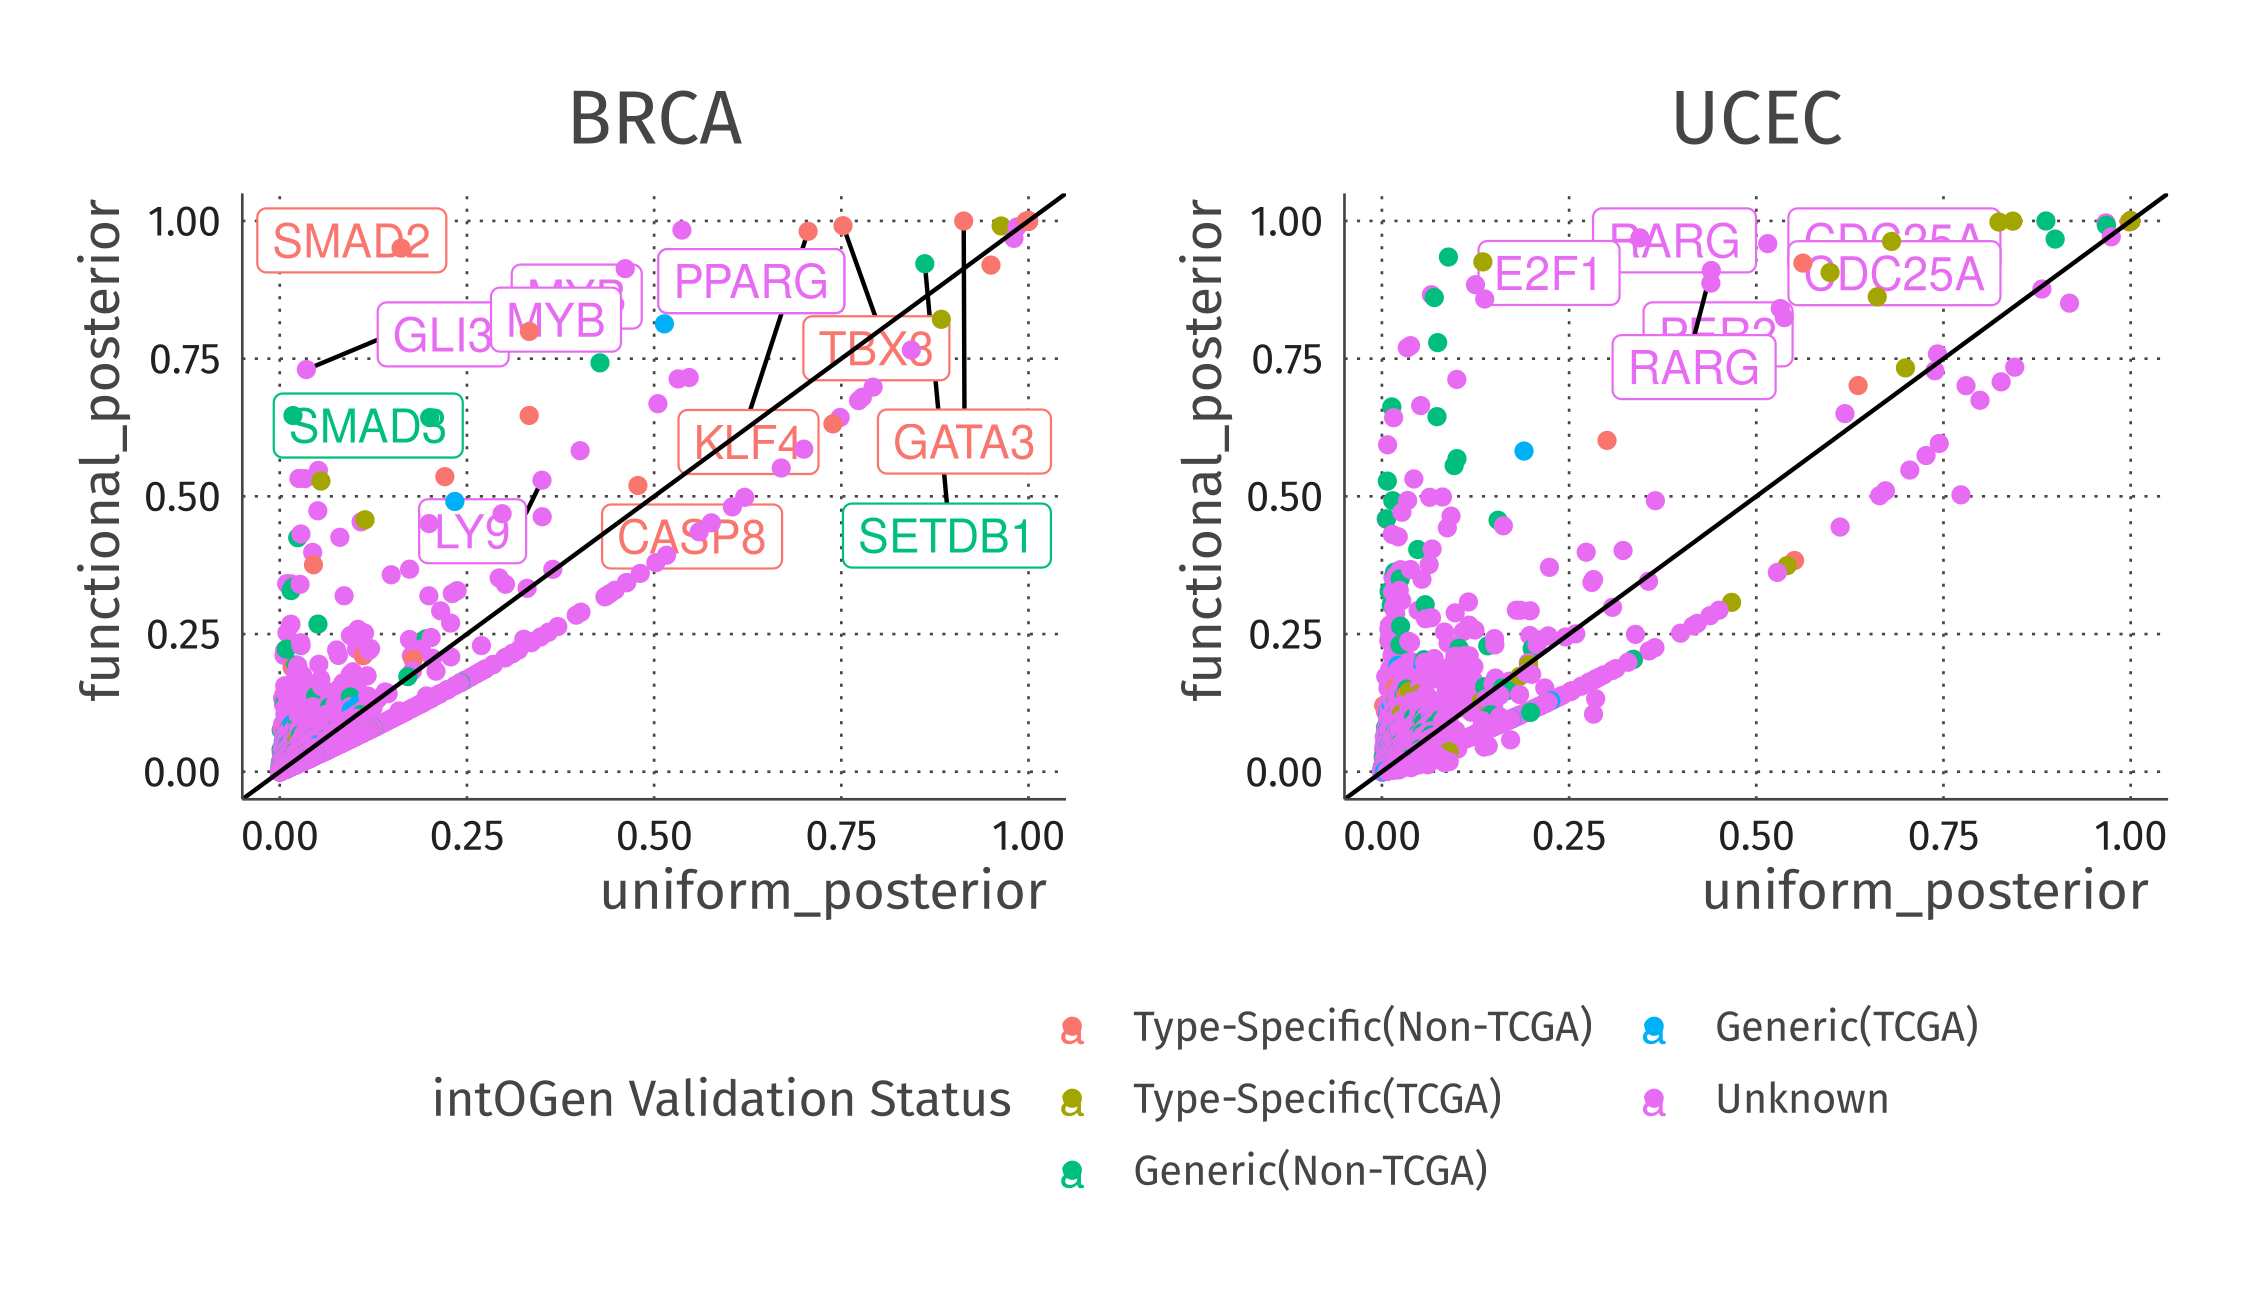
\includegraphics[width=.9\linewidth]{img/fgem_posterior_plot.png}\label{fig:fgem_posterior}
    \caption{Comparison of gene-level posterior under uniform and functional models for  Breast Invasive Carcinoma (BRCA) and Uterine Corpus Endometrial Carcinoma (UCEC).}
\end{figure}

\begin{figure}
    \centering
    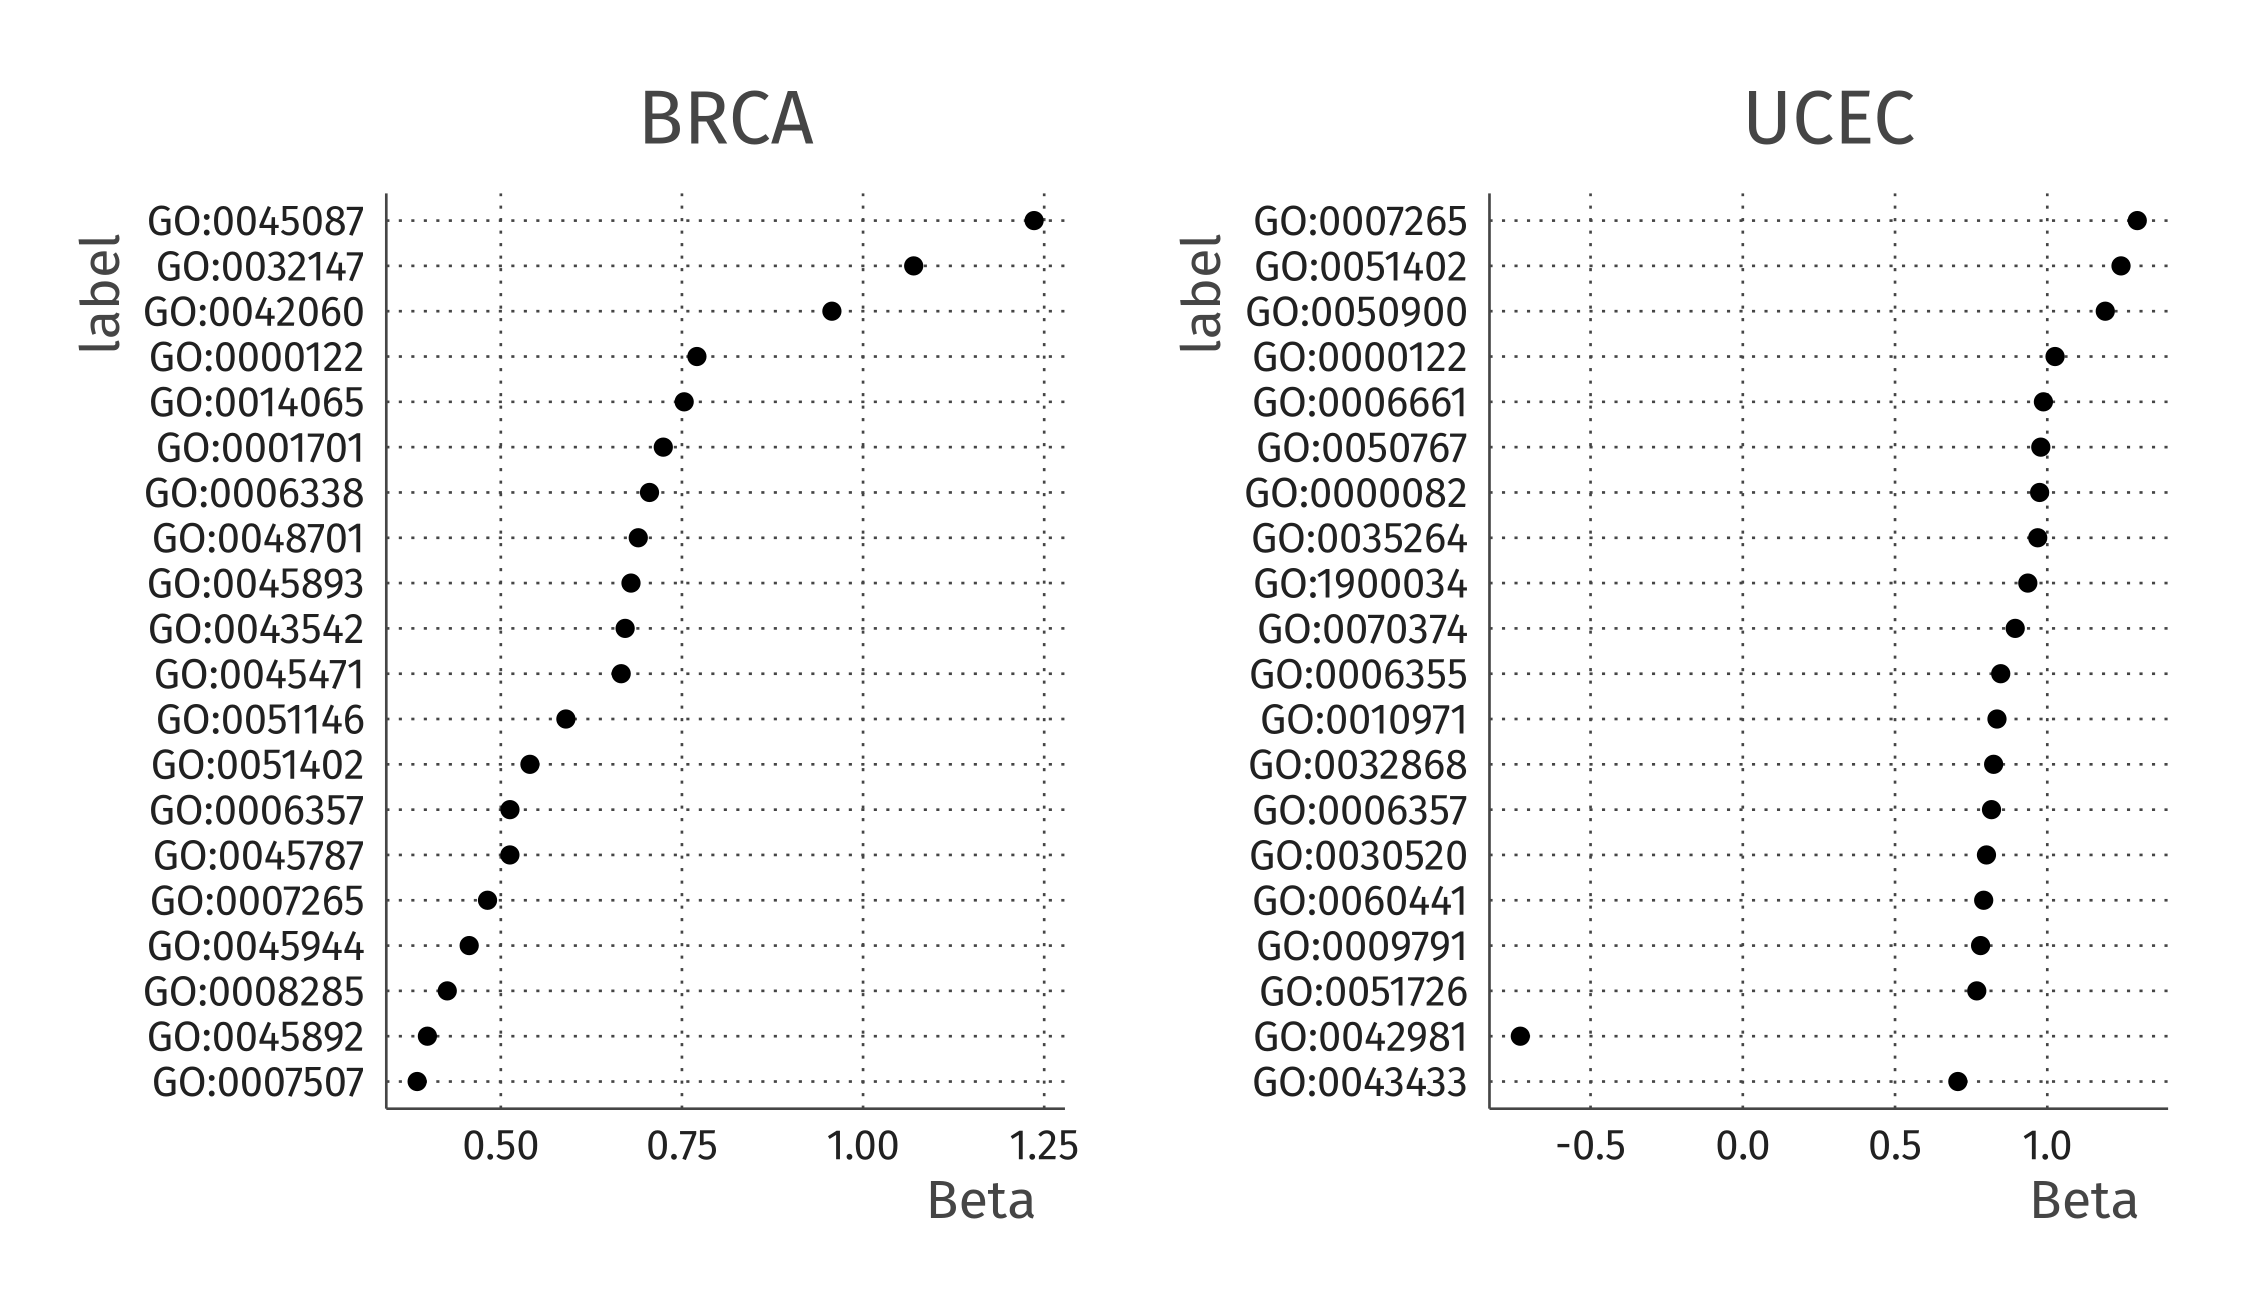
\includegraphics[width=.9\linewidth]{img/fgem_enrichment_plot.png}
    \lable{fig:fgem_enrichment}
    \caption{Multi-Feature enrichment estimate of the top 20 features (by absolute enrichment) for BRCA and UCEC.} 
\end{figure}

% \begin{figure}
%     \centering
% \begin{tabular}{l|l|r|r|r|r|l}
% \hline
% Cancer & Gene & BF & functional posterior & uniform posterior & functional prior & intOGen Validation Status\\
% \hline
% SKCM & CDKN1A & -0.1050424 & 0.9785335 & 0.0051083 & 0.9806326 & Known \\
% \hline
% PRAD & SMAD3 & 0.0166564 & 0.9914754 & 0.0196157 & 0.9913334 & Known \\
% \hline
% PAAD & BMP2 & -0.2161379 & 0.9894372 & 0.0230885 & 0.9914728 & Unknown \\
% \hline
% KIRC & TGFB1 & -0.4437373 & 0.9721332 & 0.0102885 & 0.9819394 & Unknown \\
% \hline
% LUAD & PTEN & 1.8961662 & 0.9894831 & 0.0364872 & 0.9338898 & Known \\
% \hline
% SARC & PTPRK & 0.9053713 & 0.9809541 & 0.0368396 & 0.9541875 & Known \\
% \hline
% GBM & TGFB1 & -0.3837212 & 0.9467147 & 0.0135079 & 0.9630685 & Unknown \\
% \hline
% LUSC & FBXW7 & 3.1761937 & 0.9820268 & 0.0953494 & 0.6952001 & Known Type-Specific\\
% \hline
% UCS & PARK7 & -0.0922800 & 0.8960789 & 0.0129180 & 0.9043635 & Unknown \\
% \hline
% CESC & AKT1 & 2.0105368 & 0.9891738 & 0.1181437 & 0.9244469 & Known Type-Specific \\
% \hline
% ESCA & SMARCA2 & 1.3002554 & 0.9106001 & 0.0587907 & 0.7351145 & Unknown \\
% \hline
% UCEC & PIK3CB & 1.6707522 & 0.9344572 & 0.0888288 & 0.7283980 & Known \\
% \hline
% LIHC & CDKN1A & 2.7626673 & 0.9893290 & 0.1619111 & 0.8540635 & Known Type-Specific \\
% \hline
% BRCA & SMAD2 & 2.5716367 & 0.9506715 & 0.1620579 & 0.5955677 & Known Type-Specific \\
% \hline
% BLCA & PPARG & 1.8800425 & 0.9218300 & 0.1442086 & 0.6427759 & Unknown \\
% \hline
% KIRP & MAPK1 & 0.3788399 & 0.5871487 & 0.0183591 & 0.4933381 & Known \\
% \hline
% TGCT & RAC1 & 3.9860580 & 0.7388052 & 0.1906034 & 0.0499121 & Known \\
% \hline
% \end{tabular}\label{tab:top_inc_genes}
% \caption{The gene with the highest increase in posterior probability in each cancer type, along with the status of the gene in the cancer-type specific intogen database\cite{gonzalez-perez13_intog_mutat_ident_cancer_driver}}
% \end{figure}


\subsection{Removing highly enriched single features}\label{sec:org530c0fc}

As stated in the Methods section, features with very high enrichment in single-feature analysis were removed from consideration for inclusion in the joint model. We think these very high enrichments likely reflect some identifiability problem, and are not reliable to be included in the gene prior model.  
Overall there were 233 of the 12,019 GO terms across the 18 cancer types which were excluded from the multi-feature model. Several features were excluded from a large number of cancer types, including ... %and several features that had very high average enrichment estimates
The feature with the highest significant enrichment estimate across all cancer types was GO:0045747, positive regulation of Notch signaling pathway, in TGCT.  GO:0045747 had a single-feature effect estimate of 7.412 and an FDR-adjusted $p$-value of 0.033.  Notch signaling is known to play an important role in germ cell devlopment and spermatogenesis\cite{Huang_2013}, and TGCT are widely believed to originate from human primordial germ cells\cite{baroni19_origin_testic_germ_cell_tumor}.  The relationship between Notch signaling and TGCT pathogenesis has been explored previously\cite{hayashi04_expres_failur_notch_signal_system}.

\begin{figure}
    \centering
\begin{tabular}{l|r}
  \hline
  Cancer Type & Number of highly enriched features\\
  \hline
  CESC & 43\\
  \hline
  PRAD & 42\\
  \hline
  UCEC & 34\\
  \hline
  GBM & 31\\
  \hline
  LIHC & 30\\
  \hline
  BLCA & 23\\
  \hline
  HNSC & 23\\
  \hline
  KIRC & 22\\
  \hline
  ESCA & 21\\
  \hline
  PAAD & 20\\
  \hline
  BRCA & 19\\
  \hline
  LUAD & 11\\
  \hline
  SARC & 10\\
  \hline
  LUSC & 9\\
  \hline
  TGCT & 6\\
  \hline
  UCS & 6\\
  \hline
  SKCM & 3\\
  \hline
  KIRP & 1\\
  \hline
\end{tabular}\label{fig:n_enriched}
    \caption{The number of features in each cancer type deemed ineligible for inclusion in the multi-feature enrichment method due to very high single-feature enrichment.}
\end{figure}


\section{Discussion}\label{sec:org3165b14}

We have developed a statistical model for integrating gene-level Bayes factors with gene-level annotations to simultaneously reprioritize the genes and estimate the enrichment of the features. In our analysis of gene-level Bayes factors generated from \texttt{driverMAPS} run on TCGA data, we find that the addition of gene-level features pushes 208 genes previously below a statistical signifiance threshold be novel driver genes across 18 cancer types.
One of the most salient features of FGEM as compared to other enrichment methods like Fisher's Exact test is that FGEM does not binarize data into significant vs insignificant.  For a particular gene set in a particular data set, the enrichment of Fisher's exact test is determined by the cardinality of the entries in the 2 by 2 contingency table.  In the case of Bayes factors, under Fisher's exact test, genes for which the evidence is \emph{in favor} of the null hypothesis is treated identically to genes for which the evidence is \emph{in favor} of the alternative hypothesis, but slightly below the significance cutoff. 

That the previously identified oncogenes JUN and TGFB1 showed a much high posterior probability under the functional model than the uniform models, and that these genes were not previously identified in intOGen demonstrates the value that a method capable of comprehensive integration of all forms of somatic mutation might provide in identifying cancer genes.  Both JUN and TGFB1 rely on mechanisms other than accumulation of point mutation to operate as oncogenes.  As a consequence, they will be missed by methods that rely exclusively on somatic point mutation.
It should be noted that although the FGEM analysis employed for this paper used binary gene-level features, there is nothing inherent in the method precluding inclusion of categorical or even continuous annotations.  For categorical variables (e.g encoding which, of several possible tissues, a gene is known to be expressed in) this would be
trivial: by using a reference level\cite{chambers1992statistical} and a treatment encoding (an additional indicator variable for $k-1$ of the categorical variable's $k$ levels, with the $k$th level being an implicit reference level), the enrichment estimates would have the same interpretation as log odds ratios over the ``intercept'' model.

One important caveat of the FGEM model is that it does not account for errors or uncertainty in the gene-level annotations.  While the Gene Ontology has a formal process for gene annotation, as well as a controlled vocabulary for describing the evidence underlying every gene-annotation pair, this is not true of most gene-level annotations, and even if it were, it is not clear how one might incorporate this evidence.  It is also worth considering the extent to which publication bias, or the ``file-drawer effect'' might contribute to systematic errors in gene-level annotation. It is impossible to know the number of genes that have been tested for a particular biological process or molecular function.  Gene Ontology maintains a blacklist of disallowed gene-feature relationships\cite{huntley14_under_how_why_gene_ontol}, but it captures only the most commonly misreported gene-feature relationships.  Binary gene-level annotation of a GO term ablates the distinction between a gene that has not been assessed for a particular biological process and a gene for which there is strong evidence \emph{against} it being involved in the process.


\begin{figure}
    \centering
    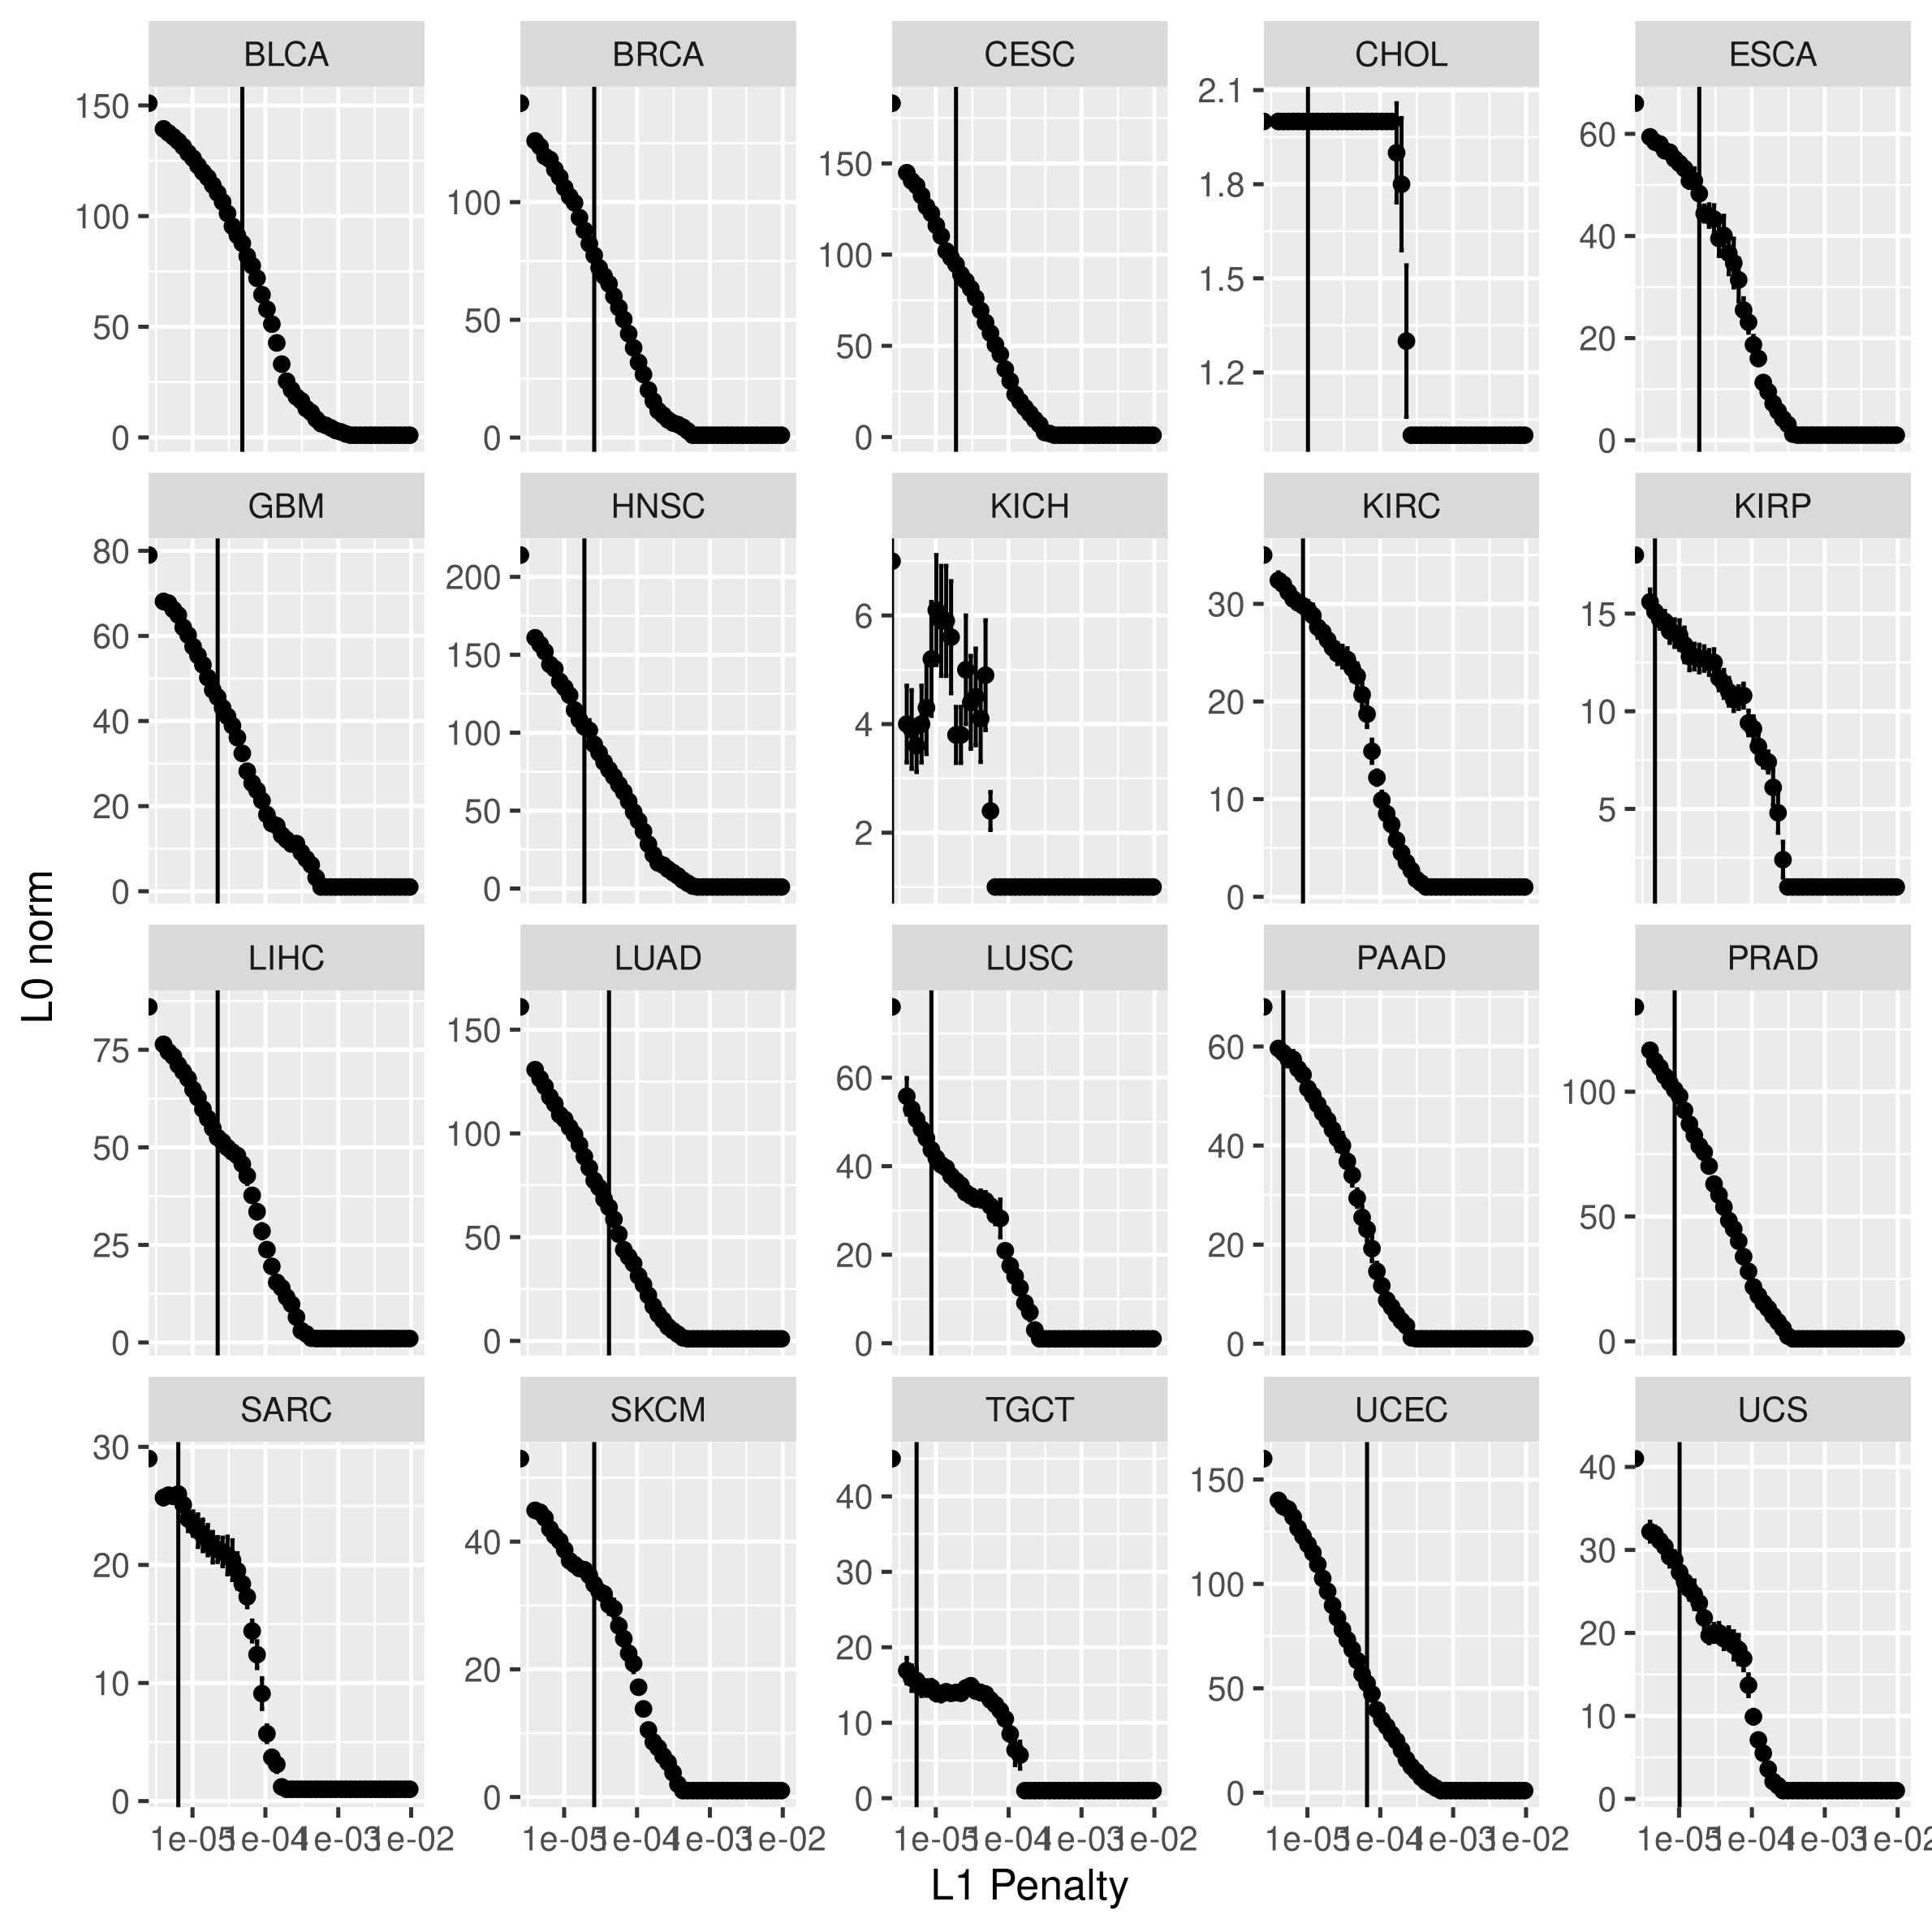
\includegraphics[width=.9\linewidth]{img/cv_l0.png}
    \label{fig:cv_l0}
    \caption{Average (over 10-fold cross-validation) number of features with non-zero effect-size estimates, as a function of $\lambda$, the elastic-net penalty, for each of 18 cancer types.}
\end{figure}

\begin{figure}
    \centering
    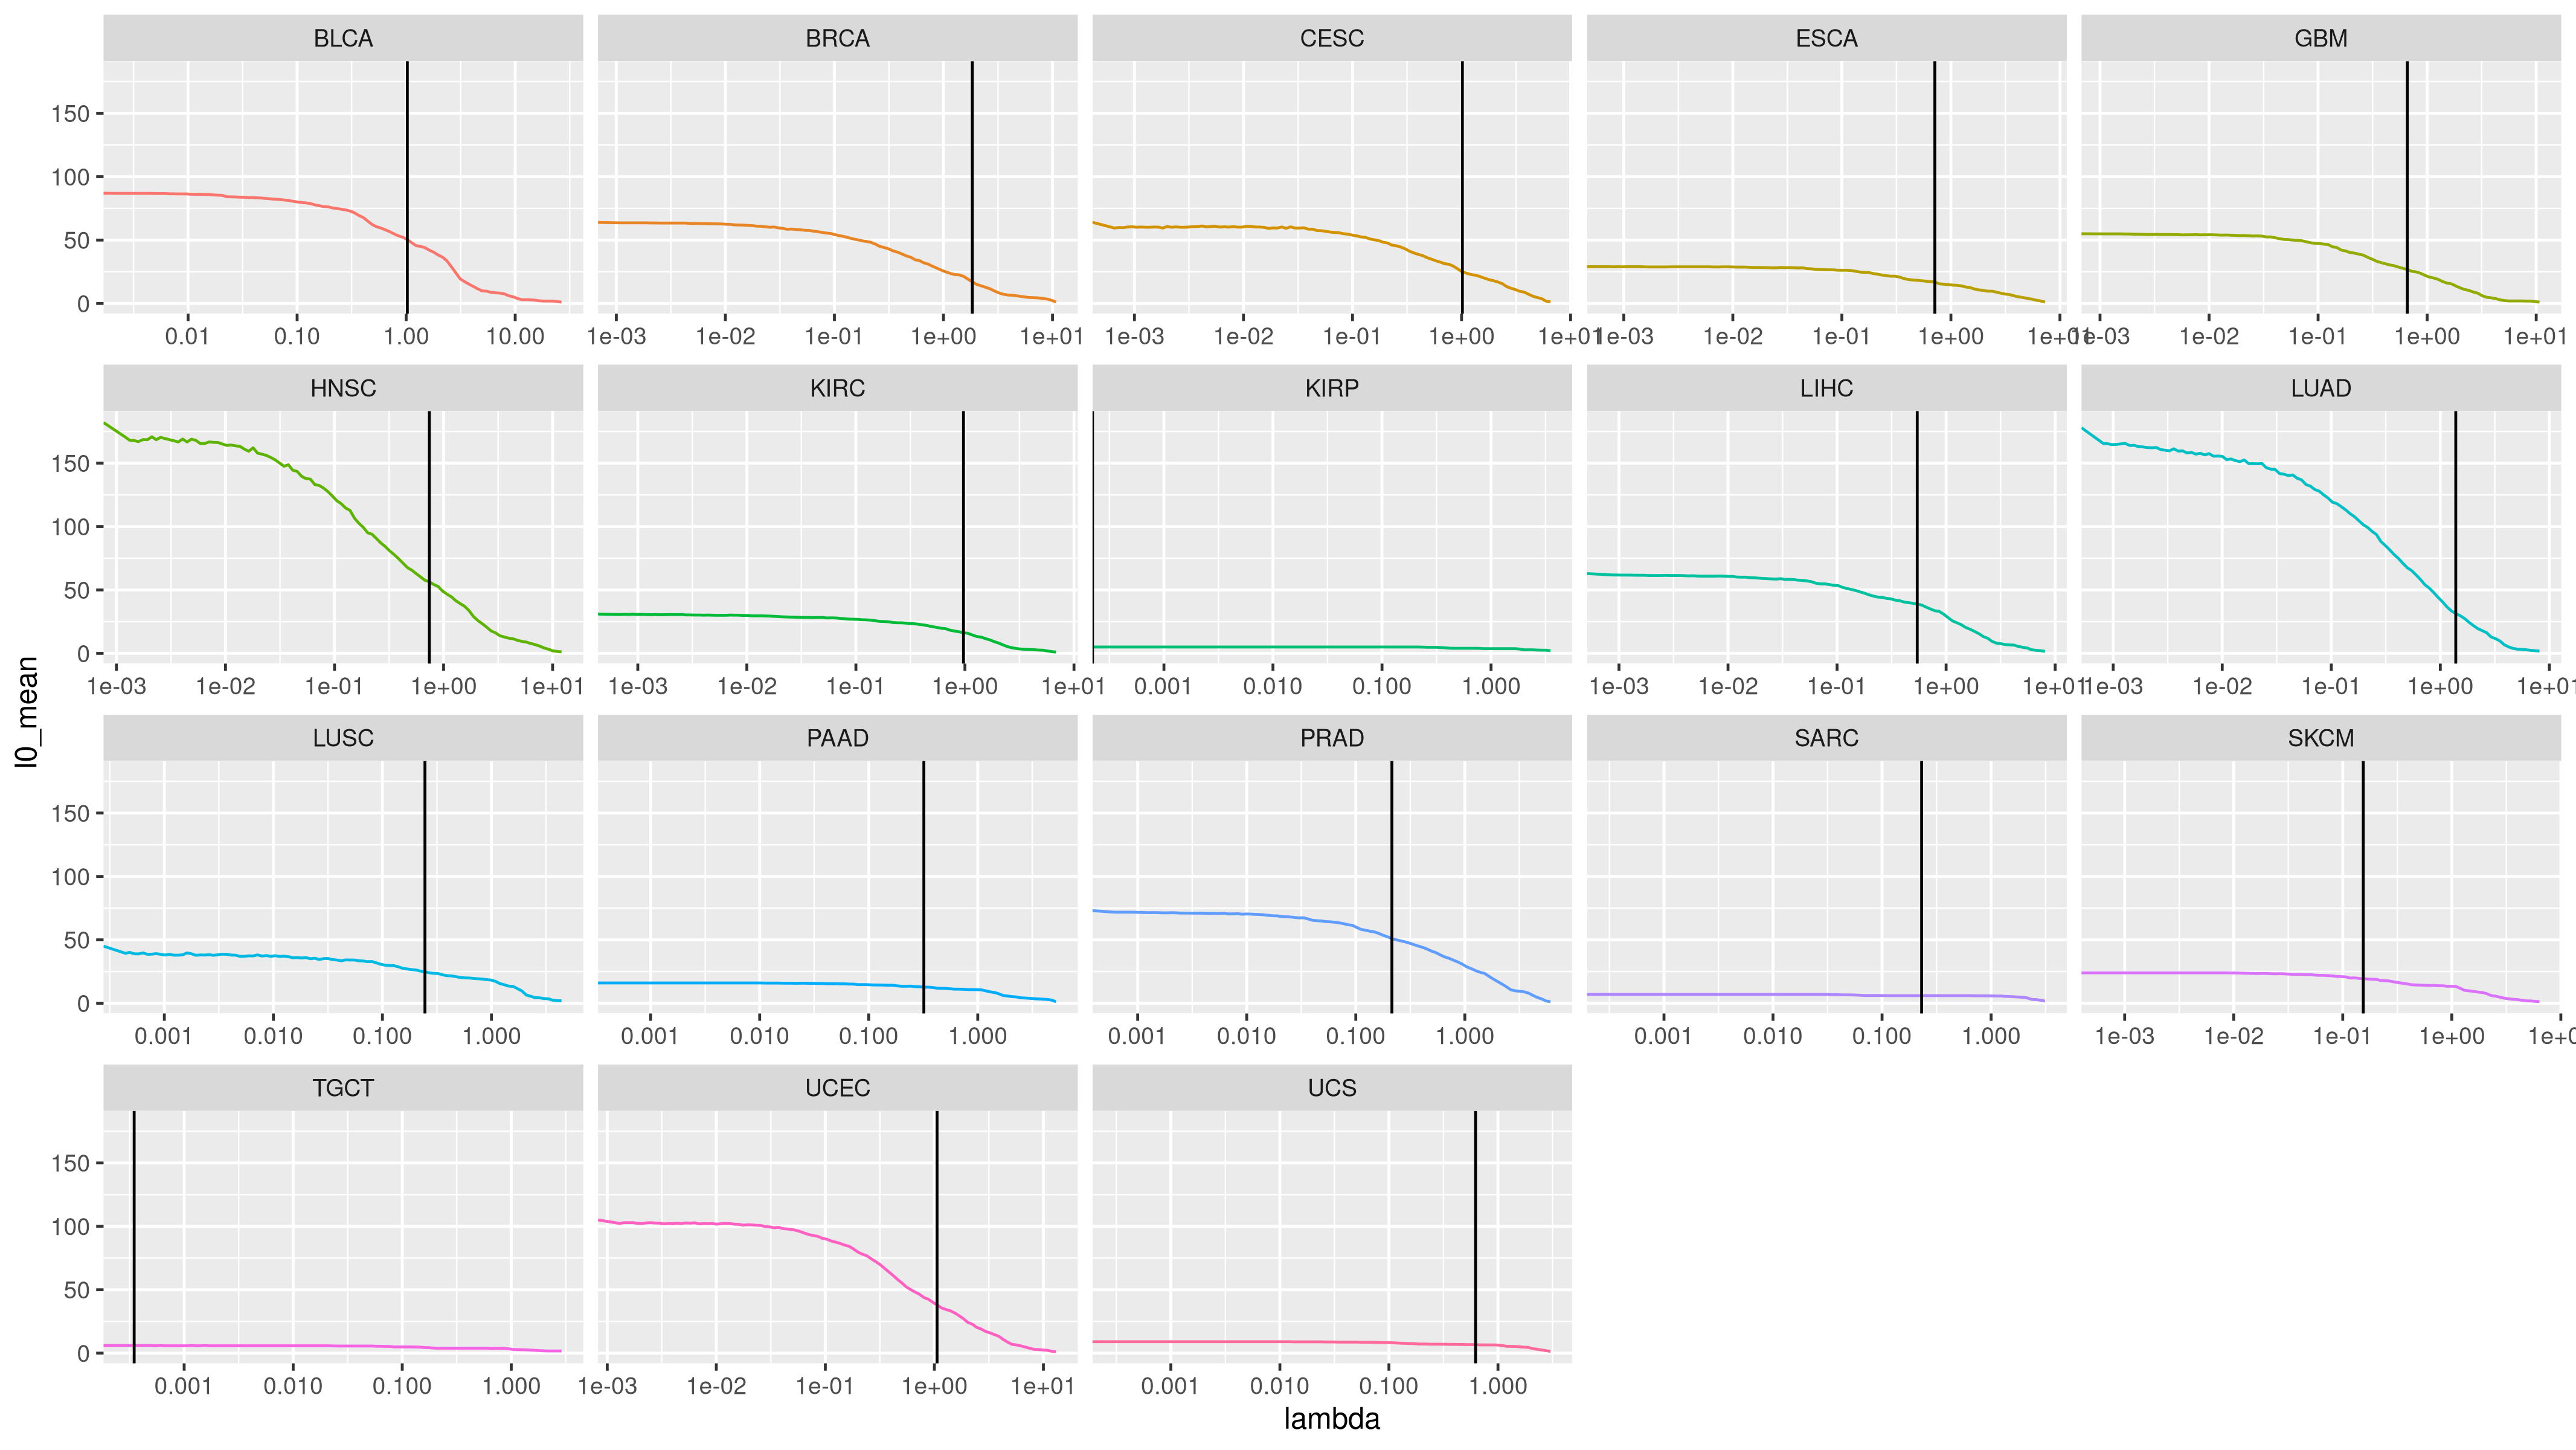
\includegraphics[width=.9\linewidth]{img/enet_cv_l0.png}
    \label{fig:enet_cv_l0}
    \caption{Average (over 10-fold cross-validation) number of features with non-zero effect-size estimates, as a function of $\lambda$, the elastic-net penalty, for each of 18 cancer types.  The vertical line
    represents the optimal value of $\lambda$.}
\end{figure}

 
 

% \bibliographystyle{unsrt}

